\documentclass[a4paper]{book}
\usepackage{makeidx}
\usepackage{graphicx}
\usepackage{multicol}
\usepackage{float}
\usepackage{listings}
\usepackage{color}
\usepackage{ifthen}
\usepackage[table]{xcolor}
\usepackage{textcomp}
\usepackage{alltt}
\usepackage[utf8]{inputenc}
\usepackage{mathptmx}
\usepackage[scaled=.90]{helvet}
\usepackage{courier}
\usepackage{sectsty}
\usepackage[titles]{tocloft}
\usepackage{doxygen}
\lstset{language=C++,inputencoding=utf8,basicstyle=\footnotesize,breaklines=true,breakatwhitespace=true,tabsize=8,numbers=left }
\makeindex
\setcounter{tocdepth}{3}
\renewcommand{\footrulewidth}{0.4pt}
\renewcommand{\familydefault}{\sfdefault}
\begin{document}
\begin{titlepage}
\vspace*{7cm}
\begin{center}
{\Large OWLTestKit \\[1ex]\large 0.1.0 }\\
\vspace*{1cm}
{\large Generated by Doxygen 1.7.4}\\
\vspace*{0.5cm}
{\small Fri May 27 2011 15:10:38}\\
\end{center}
\end{titlepage}
\clearemptydoublepage
\pagenumbering{roman}
\tableofcontents
\clearemptydoublepage
\pagenumbering{arabic}
\chapter{Module Index}
\section{Modules}
Here is a list of all modules:\begin{DoxyCompactList}
\item \contentsline{section}{Table lock type}{\pageref{group__DBDRIVER__TableLock}}{}
\item \contentsline{section}{Security bit control actions}{\pageref{group__SECURITY__BitConrol}}{}
\item \contentsline{section}{Cache areas}{\pageref{group__CACHE__Areas}}{}
\item \contentsline{section}{Query preparation types}{\pageref{group__DATA__PrepareType}}{}
\item \contentsline{section}{Dataset Reset flags}{\pageref{group__DATA__ResetFlags}}{}
\item \contentsline{section}{Return values}{\pageref{group__DBHANDLE__ReturnFlags}}{}
\item \contentsline{section}{Database handler action types}{\pageref{group__DBHANDLE__ActionTypes}}{}
\item \contentsline{section}{Database handler match types}{\pageref{group__DBHANDLE__MatchType}}{}
\item \contentsline{section}{Dataline trim flags}{\pageref{group__FILE__TrimFlags}}{}
\item \contentsline{section}{Form parse format flags}{\pageref{group__FORM__ParseFlags}}{}
\item \contentsline{section}{Dataline trim flags}{\pageref{group__FILR__TrimFlags}}{}
\item \contentsline{section}{Status code bitmaps}{\pageref{group__OWL__Bitmaps}}{}
\item \contentsline{section}{Session variable Flags}{\pageref{group__SESSION__VariableFlags}}{}
\item \contentsline{section}{Socket codes}{\pageref{group__SOCKET__Codes}}{}
\item \contentsline{section}{Application debug level}{\pageref{group__DEBUG__ApplicLevel}}{}
\item \contentsline{section}{debug levels}{\pageref{group__DEBUG__OWLLevel}}{}
\item \contentsline{section}{Severity codes}{\pageref{group__OWL__SeverityCodes}}{}
\item \contentsline{section}{Presentation modules}{\pageref{group__OWL__UI__LAYER}}{}
\item \contentsline{section}{Business Object modules}{\pageref{group__OWL__BO__LAYER}}{}
\item \contentsline{section}{Storage Object modules}{\pageref{group__OWL__SO__LAYER}}{}
\item \contentsline{section}{Library (codes, messages files etc.)}{\pageref{group__OWL__LIBRARY}}{}
\item \contentsline{section}{Plugins for the presentation modules}{\pageref{group__OWL__UI__PLUGINS}}{}
\item \contentsline{section}{Drivers}{\pageref{group__OWL__DRIVERS}}{}
\item \contentsline{section}{Global constants}{\pageref{group__OWL__Globals}}{}
\item \contentsline{section}{Global constants for the application}{\pageref{group__OWL__Application__Globals}}{}
\end{DoxyCompactList}

\chapter{Class Index}
\section{Class Hierarchy}
This inheritance list is sorted roughly, but not completely, alphabetically:\begin{DoxyCompactList}
\item \contentsline{section}{\_\-OWL}{\pageref{class__OWL}}{}
\begin{DoxyCompactList}
\item \contentsline{section}{BaseElement}{\pageref{classBaseElement}}{}
\begin{DoxyCompactList}
\item \contentsline{section}{Container}{\pageref{classContainer}}{}
\item \contentsline{section}{ContainerPlugin}{\pageref{classContainerPlugin}}{}
\begin{DoxyCompactList}
\item \contentsline{section}{ContainerDivPlugin}{\pageref{classContainerDivPlugin}}{}
\item \contentsline{section}{ContainerFieldsetPlugin}{\pageref{classContainerFieldsetPlugin}}{}
\item \contentsline{section}{ContainerItemPlugin}{\pageref{classContainerItemPlugin}}{}
\item \contentsline{section}{ContainerLabelPlugin}{\pageref{classContainerLabelPlugin}}{}
\item \contentsline{section}{ContainerLegendPlugin}{\pageref{classContainerLegendPlugin}}{}
\item \contentsline{section}{ContainerLinkPlugin}{\pageref{classContainerLinkPlugin}}{}
\item \contentsline{section}{ContainerListPlugin}{\pageref{classContainerListPlugin}}{}
\begin{DoxyCompactList}
\item \contentsline{section}{ContainerMenuPlugin}{\pageref{classContainerMenuPlugin}}{}
\end{DoxyCompactList}
\item \contentsline{section}{ContainerSpanPlugin}{\pageref{classContainerSpanPlugin}}{}
\item \contentsline{section}{ContainerTablecellPlugin}{\pageref{classContainerTablecellPlugin}}{}
\item \contentsline{section}{ContainerTablePlugin}{\pageref{classContainerTablePlugin}}{}
\item \contentsline{section}{ContainerTablerowPlugin}{\pageref{classContainerTablerowPlugin}}{}
\end{DoxyCompactList}
\item \contentsline{section}{Document}{\pageref{classDocument}}{}
\item \contentsline{section}{Form}{\pageref{classForm}}{}
\item \contentsline{section}{FormFieldPlugin}{\pageref{classFormFieldPlugin}}{}
\begin{DoxyCompactList}
\item \contentsline{section}{FormFieldButtonPlugin}{\pageref{classFormFieldButtonPlugin}}{}
\item \contentsline{section}{FormFieldCheckboxPlugin}{\pageref{classFormFieldCheckboxPlugin}}{}
\item \contentsline{section}{FormFieldFilePlugin}{\pageref{classFormFieldFilePlugin}}{}
\item \contentsline{section}{FormFieldRadioPlugin}{\pageref{classFormFieldRadioPlugin}}{}
\item \contentsline{section}{FormFieldSelectPlugin}{\pageref{classFormFieldSelectPlugin}}{}
\item \contentsline{section}{FormFieldTextareaPlugin}{\pageref{classFormFieldTextareaPlugin}}{}
\item \contentsline{section}{FormFieldTextPlugin}{\pageref{classFormFieldTextPlugin}}{}
\end{DoxyCompactList}
\end{DoxyCompactList}
\item \contentsline{section}{ContentArea}{\pageref{classContentArea}}{}
\item \contentsline{section}{DataHandler}{\pageref{classDataHandler}}{}
\begin{DoxyCompactList}
\item \contentsline{section}{HDataHandler}{\pageref{classHDataHandler}}{}
\end{DoxyCompactList}
\item \contentsline{section}{DbHandler}{\pageref{classDbHandler}}{}
\item \contentsline{section}{Dispatcher}{\pageref{classDispatcher}}{}
\item \contentsline{section}{FileHandler}{\pageref{classFileHandler}}{}
\begin{DoxyCompactList}
\item \contentsline{section}{ImageHandler}{\pageref{classImageHandler}}{}
\end{DoxyCompactList}
\item \contentsline{section}{FormHandler}{\pageref{classFormHandler}}{}
\item \contentsline{section}{Group}{\pageref{classGroup}}{}
\item \contentsline{section}{LogHandler}{\pageref{classLogHandler}}{}
\item \contentsline{section}{Mail}{\pageref{classMail}}{}
\item \contentsline{section}{OWL}{\pageref{classOWL}}{}
\item \contentsline{section}{SchemeHandler}{\pageref{classSchemeHandler}}{}
\item \contentsline{section}{SessionHandler}{\pageref{classSessionHandler}}{}
\begin{DoxyCompactList}
\item \contentsline{section}{Session}{\pageref{classSession}}{}
\end{DoxyCompactList}
\item \contentsline{section}{SocketHandler}{\pageref{classSocketHandler}}{}
\item \contentsline{section}{User}{\pageref{classUser}}{}
\end{DoxyCompactList}
\item \contentsline{section}{ConfigHandler}{\pageref{classConfigHandler}}{}
\item \contentsline{section}{DbDefaults}{\pageref{classDbDefaults}}{}
\begin{DoxyCompactList}
\item \contentsline{section}{MySQL}{\pageref{classMySQL}}{}
\end{DoxyCompactList}
\item \contentsline{section}{DbDriver}{\pageref{interfaceDbDriver}}{}
\begin{DoxyCompactList}
\item \contentsline{section}{MySQL}{\pageref{classMySQL}}{}
\end{DoxyCompactList}
\item \contentsline{section}{MailDefaults}{\pageref{classMailDefaults}}{}
\begin{DoxyCompactList}
\item \contentsline{section}{RawSMTP}{\pageref{classRawSMTP}}{}
\end{DoxyCompactList}
\item \contentsline{section}{MailDriver}{\pageref{interfaceMailDriver}}{}
\begin{DoxyCompactList}
\item \contentsline{section}{RawSMTP}{\pageref{classRawSMTP}}{}
\end{DoxyCompactList}
\item \contentsline{section}{OldOFMStuff}{\pageref{classOldOFMStuff}}{}
\item \contentsline{section}{OutputHandler}{\pageref{classOutputHandler}}{}
\item \contentsline{section}{OWLCache}{\pageref{classOWLCache}}{}
\item \contentsline{section}{OWLException}{\pageref{classOWLException}}{}
\item \contentsline{section}{OWLExceptionHandler}{\pageref{classOWLExceptionHandler}}{}
\item \contentsline{section}{OWLinstaller}{\pageref{classOWLinstaller}}{}
\item \contentsline{section}{OWLloader}{\pageref{classOWLloader}}{}
\item \contentsline{section}{OWLTimers}{\pageref{classOWLTimers}}{}
\item \contentsline{section}{Register}{\pageref{classRegister}}{}
\item \contentsline{section}{Security}{\pageref{classSecurity}}{}
\begin{DoxyCompactList}
\item \contentsline{section}{Rights}{\pageref{classRights}}{}
\end{DoxyCompactList}
\item \contentsline{section}{StatusHandler}{\pageref{classStatusHandler}}{}
\end{DoxyCompactList}

\chapter{Class Index}
\section{OWL-PHP Class List}
Here are the classes, structs, unions and interfaces with brief descriptions:\begin{CompactList}
\item\contentsline{section}{\hyperlink{class__OWL}{\_\-OWL} }{\pageref{class__OWL}}{}
\item\contentsline{section}{\hyperlink{classConfigHandler}{ConfigHandler} (Configuration handler )}{\pageref{classConfigHandler}}{}
\item\contentsline{section}{\hyperlink{classDataHandler}{DataHandler} (The \hyperlink{classOWL}{OWL} Data object )}{\pageref{classDataHandler}}{}
\item\contentsline{section}{\hyperlink{classDbHandler}{DbHandler} (Database handler )}{\pageref{classDbHandler}}{}
\item\contentsline{section}{\hyperlink{classFileHandler}{FileHandler} (File handler )}{\pageref{classFileHandler}}{}
\item\contentsline{section}{\hyperlink{classFormHandler}{FormHandler} (Formhandler )}{\pageref{classFormHandler}}{}
\item\contentsline{section}{\hyperlink{classLogHandler}{LogHandler} (Log handler )}{\pageref{classLogHandler}}{}
\item\contentsline{section}{\hyperlink{classOWL}{OWL} }{\pageref{classOWL}}{}
\item\contentsline{section}{\hyperlink{classOWLException}{OWLException} (Exception handler )}{\pageref{classOWLException}}{}
\item\contentsline{section}{\hyperlink{classOWLExceptionHandler}{OWLExceptionHandler} (Default exception handler )}{\pageref{classOWLExceptionHandler}}{}
\item\contentsline{section}{\hyperlink{classRegister}{Register} }{\pageref{classRegister}}{}
\item\contentsline{section}{\hyperlink{classSession}{Session} (OWL-PHP session object )}{\pageref{classSession}}{}
\item\contentsline{section}{\hyperlink{classSessionHandler}{SessionHandler} (PHP session object )}{\pageref{classSessionHandler}}{}
\item\contentsline{section}{\hyperlink{classStatusHandler}{StatusHandler} (Status object )}{\pageref{classStatusHandler}}{}
\item\contentsline{section}{\hyperlink{classUser}{User} (OWL-PHP session object )}{\pageref{classUser}}{}
\item\contentsline{section}{\hyperlink{classUserHandler}{UserHandler} (\hyperlink{classUser}{User} object )}{\pageref{classUserHandler}}{}
\end{CompactList}

\chapter{File Index}
\section{File List}
Here is a list of all files with brief descriptions:\begin{DoxyCompactList}
\item\contentsline{section}{/home/oscar/projects/owl-\/php/src/\hyperlink{config_8php}{config.php} }{\pageref{config_8php}}{}
\item\contentsline{section}{/home/oscar/projects/owl-\/php/src/\hyperlink{index_8php}{index.php} }{\pageref{index_8php}}{}
\item\contentsline{section}{/home/oscar/projects/owl-\/php/src/\hyperlink{OWLloader_8php}{OWLloader.php} }{\pageref{OWLloader_8php}}{}
\item\contentsline{section}{/home/oscar/projects/owl-\/php/src/\hyperlink{OWLrundown_8php}{OWLrundown.php} }{\pageref{OWLrundown_8php}}{}
\item\contentsline{section}{/home/oscar/projects/owl-\/php/src/kernel/\hyperlink{class_8__owl_8php}{class.\_\-owl.php} }{\pageref{class_8__owl_8php}}{}
\item\contentsline{section}{/home/oscar/projects/owl-\/php/src/kernel/bo/\hyperlink{class_8dispatcher_8php}{class.dispatcher.php} }{\pageref{class_8dispatcher_8php}}{}
\item\contentsline{section}{/home/oscar/projects/owl-\/php/src/kernel/bo/\hyperlink{class_8form_8php}{class.form.php} }{\pageref{class_8form_8php}}{}
\item\contentsline{section}{/home/oscar/projects/owl-\/php/src/kernel/bo/\hyperlink{class_8owl_8php}{class.owl.php} }{\pageref{class_8owl_8php}}{}
\item\contentsline{section}{/home/oscar/projects/owl-\/php/src/kernel/bo/\hyperlink{class_8session_8php}{class.session.php} }{\pageref{class_8session_8php}}{}
\item\contentsline{section}{/home/oscar/projects/owl-\/php/src/kernel/bo/\hyperlink{class_8user_8php}{class.user.php} }{\pageref{class_8user_8php}}{}
\item\contentsline{section}{/home/oscar/projects/owl-\/php/src/kernel/so/\hyperlink{class_8confighandler_8php}{class.confighandler.php} }{\pageref{class_8confighandler_8php}}{}
\item\contentsline{section}{/home/oscar/projects/owl-\/php/src/kernel/so/\hyperlink{class_8datahandler_8php}{class.datahandler.php} }{\pageref{class_8datahandler_8php}}{}
\item\contentsline{section}{/home/oscar/projects/owl-\/php/src/kernel/so/\hyperlink{class_8dbhandler_8php}{class.dbhandler.php} }{\pageref{class_8dbhandler_8php}}{}
\item\contentsline{section}{/home/oscar/projects/owl-\/php/src/kernel/so/\hyperlink{class_8exceptionhandler_8php}{class.exceptionhandler.php} }{\pageref{class_8exceptionhandler_8php}}{}
\item\contentsline{section}{/home/oscar/projects/owl-\/php/src/kernel/so/\hyperlink{class_8filehandler_8php}{class.filehandler.php} }{\pageref{class_8filehandler_8php}}{}
\item\contentsline{section}{/home/oscar/projects/owl-\/php/src/kernel/so/\hyperlink{class_8formhandler_8php}{class.formhandler.php} }{\pageref{class_8formhandler_8php}}{}
\item\contentsline{section}{/home/oscar/projects/owl-\/php/src/kernel/so/\hyperlink{class_8imagehandler_8php}{class.imagehandler.php} }{\pageref{class_8imagehandler_8php}}{}
\item\contentsline{section}{/home/oscar/projects/owl-\/php/src/kernel/so/\hyperlink{class_8loghandler_8php}{class.loghandler.php} }{\pageref{class_8loghandler_8php}}{}
\item\contentsline{section}{/home/oscar/projects/owl-\/php/src/kernel/so/\hyperlink{class_8register_8php}{class.register.php} }{\pageref{class_8register_8php}}{}
\item\contentsline{section}{/home/oscar/projects/owl-\/php/src/kernel/so/\hyperlink{class_8schemehandler_8php}{class.schemehandler.php} }{\pageref{class_8schemehandler_8php}}{}
\item\contentsline{section}{/home/oscar/projects/owl-\/php/src/kernel/so/\hyperlink{class_8sessionhandler_8php}{class.sessionhandler.php} }{\pageref{class_8sessionhandler_8php}}{}
\item\contentsline{section}{/home/oscar/projects/owl-\/php/src/kernel/so/\hyperlink{class_8statushandler_8php}{class.statushandler.php} }{\pageref{class_8statushandler_8php}}{}
\item\contentsline{section}{/home/oscar/projects/owl-\/php/src/kernel/so/\hyperlink{class_8userhandler_8php}{class.userhandler.php} }{\pageref{class_8userhandler_8php}}{}
\item\contentsline{section}{/home/oscar/projects/owl-\/php/src/kernel/ui/\hyperlink{class_8baseelement_8php}{class.baseelement.php} }{\pageref{class_8baseelement_8php}}{}
\item\contentsline{section}{/home/oscar/projects/owl-\/php/src/kernel/ui/\hyperlink{class_8formfield_8php}{class.formfield.php} }{\pageref{class_8formfield_8php}}{}
\item\contentsline{section}{/home/oscar/projects/owl-\/php/src/kernel/ui/formfields/\hyperlink{class_8formfield_8button_8php}{class.formfield.button.php} }{\pageref{class_8formfield_8button_8php}}{}
\item\contentsline{section}{/home/oscar/projects/owl-\/php/src/kernel/ui/formfields/\hyperlink{class_8formfield_8checkbox_8php}{class.formfield.checkbox.php} }{\pageref{class_8formfield_8checkbox_8php}}{}
\item\contentsline{section}{/home/oscar/projects/owl-\/php/src/kernel/ui/formfields/\hyperlink{class_8formfield_8file_8php}{class.formfield.file.php} }{\pageref{class_8formfield_8file_8php}}{}
\item\contentsline{section}{/home/oscar/projects/owl-\/php/src/kernel/ui/formfields/\hyperlink{class_8formfield_8radio_8php}{class.formfield.radio.php} }{\pageref{class_8formfield_8radio_8php}}{}
\item\contentsline{section}{/home/oscar/projects/owl-\/php/src/kernel/ui/formfields/\hyperlink{class_8formfield_8select_8php}{class.formfield.select.php} }{\pageref{class_8formfield_8select_8php}}{}
\item\contentsline{section}{/home/oscar/projects/owl-\/php/src/kernel/ui/formfields/\hyperlink{class_8formfield_8text_8php}{class.formfield.text.php} }{\pageref{class_8formfield_8text_8php}}{}
\item\contentsline{section}{/home/oscar/projects/owl-\/php/src/kernel/ui/formfields/\hyperlink{class_8formfield_8textarea_8php}{class.formfield.textarea.php} }{\pageref{class_8formfield_8textarea_8php}}{}
\item\contentsline{section}{/home/oscar/projects/owl-\/php/src/lib/\hyperlink{owl_8debug_8functions_8php}{owl.debug.functions.php} }{\pageref{owl_8debug_8functions_8php}}{}
\item\contentsline{section}{/home/oscar/projects/owl-\/php/src/lib/\hyperlink{owl_8helper_8functions_8php}{owl.helper.functions.php} }{\pageref{owl_8helper_8functions_8php}}{}
\item\contentsline{section}{/home/oscar/projects/owl-\/php/src/lib/\hyperlink{owl_8messages_8en-uk_8php}{owl.messages.en-\/uk.php} }{\pageref{owl_8messages_8en-uk_8php}}{}
\item\contentsline{section}{/home/oscar/projects/owl-\/php/src/lib/\hyperlink{owl_8messages_8php}{owl.messages.php} }{\pageref{owl_8messages_8php}}{}
\item\contentsline{section}{/home/oscar/projects/owl-\/php/src/lib/\hyperlink{owl_8nodebug_8functions_8php}{owl.nodebug.functions.php} }{\pageref{owl_8nodebug_8functions_8php}}{}
\item\contentsline{section}{/home/oscar/projects/owl-\/php/src/lib/\hyperlink{owl_8severitycodes_8php}{owl.severitycodes.php} }{\pageref{owl_8severitycodes_8php}}{}
\end{DoxyCompactList}

\chapter{Module Documentation}
\section{Test result code}
\label{group__Test__Results}\index{Test result code@{Test result code}}
\subsection*{Enumerations}
\begin{DoxyCompactItemize}
\item 
enum {\bf OTK\_\-RESULT\_\-FAIL} 
\begin{DoxyCompactList}\small\item\em Testcase ended with a failure. \end{DoxyCompactList}\item 
enum {\bf OTK\_\-RESULT\_\-SUCCESS} 
\begin{DoxyCompactList}\small\item\em The testscase ended successfully. \end{DoxyCompactList}\item 
enum {\bf OTK\_\-RESULT\_\-WARNING} 
\begin{DoxyCompactList}\small\item\em The testcase ended with a warning. \end{DoxyCompactList}\item 
enum {\bf OTK\_\-RESULT\_\-SKIPPED} 
\begin{DoxyCompactList}\small\item\em The testcase was skipped as a result of an earlier failure or warning. \end{DoxyCompactList}\item 
enum {\bf OTK\_\-RESULT\_\-NONE} 
\begin{DoxyCompactList}\small\item\em The teststep had nothing to do, ignore it. This code is reserved for prepareTest() and cleanupTest() \end{DoxyCompactList}\end{DoxyCompactItemize}


\subsection{Detailed Description}
These codes define valid return values for the steps in the testcases 

\subsection{Enumeration Type Documentation}
\index{Test result code@{Test result code}!OTK\_\-RESULT\_\-FAIL@{OTK\_\-RESULT\_\-FAIL}}
\index{OTK\_\-RESULT\_\-FAIL@{OTK\_\-RESULT\_\-FAIL}!Test result code@{Test result code}}
\subsubsection[{OTK\_\-RESULT\_\-FAIL}]{\setlength{\rightskip}{0pt plus 5cm}enum {\bf OTK\_\-RESULT\_\-FAIL}}\label{group__Test__Results_gaeb82ae39d76794b6ba8ff719fb456f06}


Testcase ended with a failure. 

\index{Test result code@{Test result code}!OTK\_\-RESULT\_\-NONE@{OTK\_\-RESULT\_\-NONE}}
\index{OTK\_\-RESULT\_\-NONE@{OTK\_\-RESULT\_\-NONE}!Test result code@{Test result code}}
\subsubsection[{OTK\_\-RESULT\_\-NONE}]{\setlength{\rightskip}{0pt plus 5cm}enum {\bf OTK\_\-RESULT\_\-NONE}}\label{group__Test__Results_gac4a467b8c7025f04e4915877cf7626eb}


The teststep had nothing to do, ignore it. This code is reserved for prepareTest() and cleanupTest() 

\index{Test result code@{Test result code}!OTK\_\-RESULT\_\-SKIPPED@{OTK\_\-RESULT\_\-SKIPPED}}
\index{OTK\_\-RESULT\_\-SKIPPED@{OTK\_\-RESULT\_\-SKIPPED}!Test result code@{Test result code}}
\subsubsection[{OTK\_\-RESULT\_\-SKIPPED}]{\setlength{\rightskip}{0pt plus 5cm}enum {\bf OTK\_\-RESULT\_\-SKIPPED}}\label{group__Test__Results_gaff709930ec00f9e05e0b93fa421e214e}


The testcase was skipped as a result of an earlier failure or warning. 

\index{Test result code@{Test result code}!OTK\_\-RESULT\_\-SUCCESS@{OTK\_\-RESULT\_\-SUCCESS}}
\index{OTK\_\-RESULT\_\-SUCCESS@{OTK\_\-RESULT\_\-SUCCESS}!Test result code@{Test result code}}
\subsubsection[{OTK\_\-RESULT\_\-SUCCESS}]{\setlength{\rightskip}{0pt plus 5cm}enum {\bf OTK\_\-RESULT\_\-SUCCESS}}\label{group__Test__Results_ga3edb448eb67c540e4343ec5797555604}


The testscase ended successfully. 

\index{Test result code@{Test result code}!OTK\_\-RESULT\_\-WARNING@{OTK\_\-RESULT\_\-WARNING}}
\index{OTK\_\-RESULT\_\-WARNING@{OTK\_\-RESULT\_\-WARNING}!Test result code@{Test result code}}
\subsubsection[{OTK\_\-RESULT\_\-WARNING}]{\setlength{\rightskip}{0pt plus 5cm}enum {\bf OTK\_\-RESULT\_\-WARNING}}\label{group__Test__Results_ga90bcc995d175f83e3c5dc29597b35819}


The testcase ended with a warning. 


\section{Presentation modules}
\label{group__OTK__UI__LAYER}\index{Presentation modules@{Presentation modules}}
\subsection*{Classes}
\begin{DoxyCompactItemize}
\item 
class {\bf MainmenuArea}
\begin{DoxyCompactList}\small\item\em Main manu. \end{DoxyCompactList}\end{DoxyCompactItemize}
\subsection*{Files}
\begin{DoxyCompactItemize}
\item 
file {\bf mainmenu.php}
\item 
file {\bf mainpage.php}
\item 
file {\bf testresults.php}
\item 
file {\bf testsets.php}
\end{DoxyCompactItemize}

\section{Business Object modules}
\label{group__OTK__BO__LAYER}\index{Business Object modules@{Business Object modules}}
\subsection*{Classes}
\begin{DoxyCompactItemize}
\item 
class {\bf OTKUser}
\begin{DoxyCompactList}\small\item\em \doxyref{OTK}{p.}{classOTK} User. \end{DoxyCompactList}\end{DoxyCompactItemize}

\section{Storage Object modules}
\label{group__OTK__SO__LAYER}\index{Storage Object modules@{Storage Object modules}}

\section{Library (codes, messages files etc.)}
\label{group__OTK__LIBRARY}\index{Library (codes, messages files etc.)@{Library (codes, messages files etc.)}}
\subsection*{Files}
\begin{DoxyCompactItemize}
\item 
file {\bf otk.applic.loader.php}
\item 
file {\bf otk.labels.php}
\item 
file {\bf otk.messages.php}
\end{DoxyCompactItemize}

\section{Administrator section}
\label{group__OTK__ADMIN}\index{Administrator section@{Administrator section}}
\subsection*{Files}
\begin{DoxyCompactItemize}
\item 
file {\bf install.php}
\end{DoxyCompactItemize}

\section{Test sets}
\label{group__OTK__TESTSETS}\index{Test sets@{Test sets}}
\subsection*{Classes}
\begin{DoxyCompactItemize}
\item 
class {\bf OTKHdata\_\-First}
\begin{DoxyCompactList}\small\item\em HData Testcase. \end{DoxyCompactList}\item 
class {\bf OTKHdata}
\begin{DoxyCompactList}\small\item\em HDataHandler testset. \end{DoxyCompactList}\end{DoxyCompactItemize}
\subsection*{Files}
\begin{DoxyCompactItemize}
\item 
file {\bf helper.php}
\end{DoxyCompactItemize}

\section{Test cases}
\label{group__OTK__TESTCASES}\index{Test cases@{Test cases}}

\chapter{Class Documentation}
\section{MainmenuArea Class Reference}
\label{classMainmenuArea}\index{MainmenuArea@{MainmenuArea}}


Main manu.  


\subsection*{Public Member Functions}
\begin{DoxyCompactItemize}
\item 
{\bf loadArea} (\$arg=null)
\end{DoxyCompactItemize}


\subsection{Detailed Description}
Main manu. 

Setup the contentarea holding the main menu \begin{DoxyAuthor}{Author}
Oscar van Eijk, Oveas Functionality Provider 
\end{DoxyAuthor}
\begin{DoxyVersion}{Version}
May 19, 2011 -\/-\/ O van Eijk -\/-\/ initial version 
\end{DoxyVersion}


\subsection{Member Function Documentation}
\index{MainmenuArea@{MainmenuArea}!loadArea@{loadArea}}
\index{loadArea@{loadArea}!MainmenuArea@{MainmenuArea}}
\subsubsection[{loadArea}]{\setlength{\rightskip}{0pt plus 5cm}MainmenuArea::loadArea (
\begin{DoxyParamCaption}
\item[{\$}]{arg = {\ttfamily null}}
\end{DoxyParamCaption}
)}\label{classMainmenuArea_ab38be841a2daec49a57e809bedba023b}
Generate the link 
\begin{DoxyParams}[1]{Parameters}
\mbox{\tt in}  & {\em \$arg} & Not used here, but required by syntax \\
\hline
\end{DoxyParams}


The documentation for this class was generated from the following file:\begin{DoxyCompactItemize}
\item 
/home/oscar/projects/owl-\/php/owltestkit/ui/{\bf mainmenu.php}\end{DoxyCompactItemize}

\section{OTK Class Reference}
\label{classOTK}\index{OTK@{OTK}}


\doxyref{OTK}{p.}{classOTK} mainclass.  


\subsection*{Public Member Functions}
\begin{DoxyCompactItemize}
\item 
{\bf \_\-\_\-construct} ()
\item 
{\bf selectTestCases} ()
\item 
{\bf doTests} ()
\end{DoxyCompactItemize}
\subsection*{Private Attributes}
\begin{DoxyCompactItemize}
\item 
{\bf \$testKit}
\end{DoxyCompactItemize}


\subsection{Detailed Description}
\doxyref{OTK}{p.}{classOTK} mainclass. 

Class that contains all methods that will be called by the OWL dispatchers \begin{DoxyAuthor}{Author}
Oscar van Eijk, Oveas Functionality Provider 
\end{DoxyAuthor}
\begin{DoxyVersion}{Version}
May 19, 2011 -\/-\/ O van Eijk -\/-\/ initial version 
\end{DoxyVersion}


\subsection{Constructor \& Destructor Documentation}
\index{OTK@{OTK}!\_\-\_\-construct@{\_\-\_\-construct}}
\index{\_\-\_\-construct@{\_\-\_\-construct}!OTK@{OTK}}
\subsubsection[{\_\-\_\-construct}]{\setlength{\rightskip}{0pt plus 5cm}OTK::\_\-\_\-construct (
\begin{DoxyParamCaption}
{}
\end{DoxyParamCaption}
)}\label{classOTK_a9a05ec6dd02b4dc6574473a812888480}
Class constructor \begin{DoxyAuthor}{Author}
Oscar van Eijk, Oveas Functionality Provider 
\end{DoxyAuthor}


\subsection{Member Function Documentation}
\index{OTK@{OTK}!doTests@{doTests}}
\index{doTests@{doTests}!OTK@{OTK}}
\subsubsection[{doTests}]{\setlength{\rightskip}{0pt plus 5cm}OTK::doTests (
\begin{DoxyParamCaption}
{}
\end{DoxyParamCaption}
)}\label{classOTK_a52498e87de15d4b6aff1d932fbbfbb64}
Read from the formdata which testsets must be executed and perform those tests. \begin{DoxyAuthor}{Author}
Oscar van Eijk, Oveas Functionality Provider 
\end{DoxyAuthor}


References \$\_\-form.

\index{OTK@{OTK}!selectTestCases@{selectTestCases}}
\index{selectTestCases@{selectTestCases}!OTK@{OTK}}
\subsubsection[{selectTestCases}]{\setlength{\rightskip}{0pt plus 5cm}OTK::selectTestCases (
\begin{DoxyParamCaption}
{}
\end{DoxyParamCaption}
)}\label{classOTK_a192cccba7a56fb485fc576f5f5afdc76}
Load the area from which the testsets can be selected for execution \begin{DoxyAuthor}{Author}
Oscar van Eijk, Oveas Functionality Provider 
\end{DoxyAuthor}


References \$GLOBALS.



\subsection{Member Data Documentation}
\index{OTK@{OTK}!\$testKit@{\$testKit}}
\index{\$testKit@{\$testKit}!OTK@{OTK}}
\subsubsection[{\$testKit}]{\setlength{\rightskip}{0pt plus 5cm}OTK::\$testKit\hspace{0.3cm}{\ttfamily  [private]}}\label{classOTK_a0e26e36f48d1ad26dcefe8528b7f32e7}
Reference to the Testkit containerobject 

The documentation for this class was generated from the following file:\begin{DoxyCompactItemize}
\item 
/home/oscar/projects/owl-\/php/owltestkit/bo/{\bf class.otk.php}\end{DoxyCompactItemize}

\section{OTKHdata Class Reference}
\label{classOTKHdata}\index{OTKHdata@{OTKHdata}}


HDataHandler testset.  


Inheritance diagram for OTKHdata:\begin{figure}[H]
\begin{center}
\leavevmode
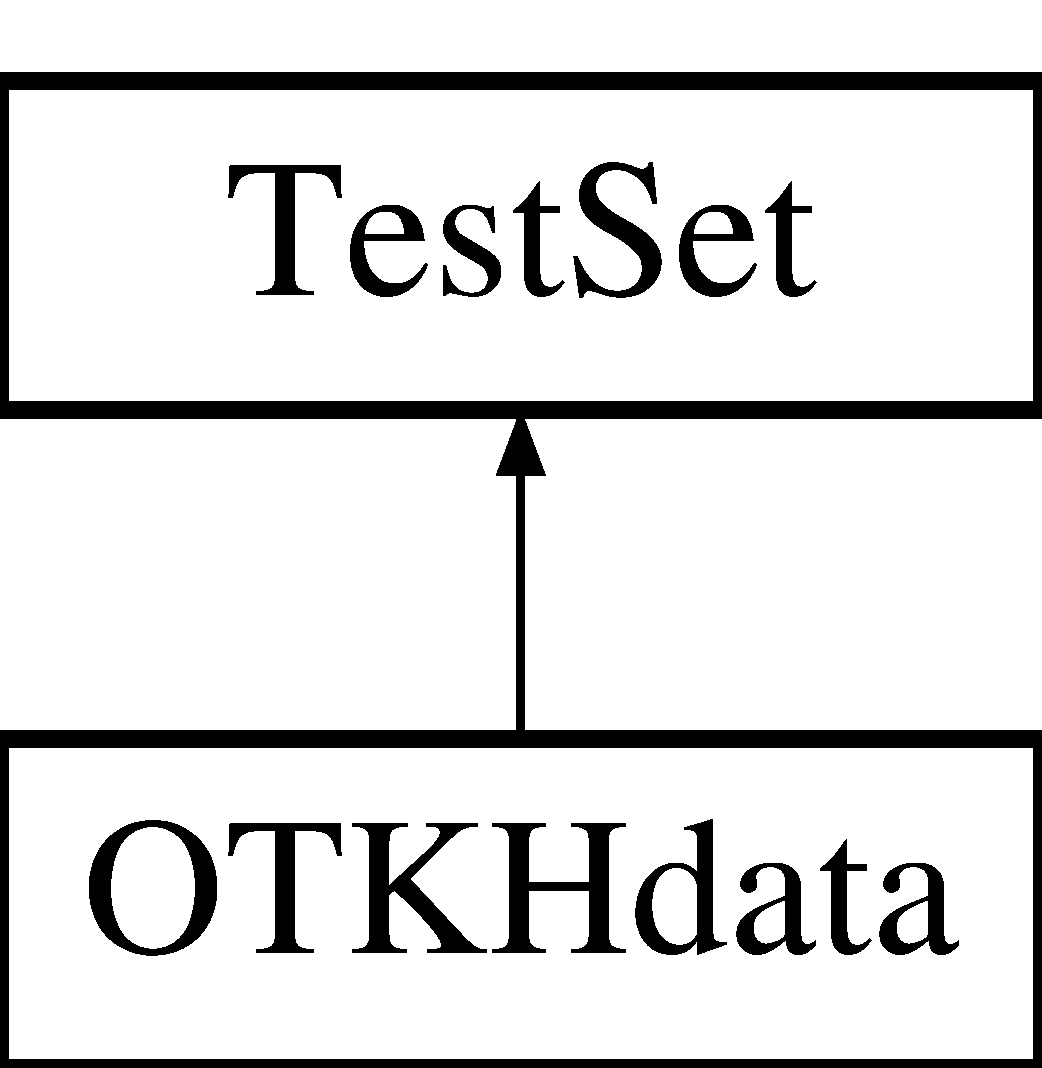
\includegraphics[height=2.000000cm]{classOTKHdata}
\end{center}
\end{figure}
\subsection*{Public Member Functions}
\begin{DoxyCompactItemize}
\item 
{\bf loadTestcases} (\$location)
\item 
{\bf performTests} ()
\end{DoxyCompactItemize}
\subsection*{Static Public Member Functions}
\begin{DoxyCompactItemize}
\item 
static {\bf getDescription} ()
\end{DoxyCompactItemize}


\subsection{Detailed Description}
HDataHandler testset. 

This class defines the testsets for the hierarchical data handler. \begin{DoxyAuthor}{Author}
Oscar van Eijk, Oveas Functionality Provider 
\end{DoxyAuthor}
\begin{DoxyVersion}{Version}
May 19, 2011 -\/-\/ O van Eijk -\/-\/ initial version 
\end{DoxyVersion}


\subsection{Member Function Documentation}
\index{OTKHdata@{OTKHdata}!getDescription@{getDescription}}
\index{getDescription@{getDescription}!OTKHdata@{OTKHdata}}
\subsubsection[{getDescription}]{\setlength{\rightskip}{0pt plus 5cm}static OTKHdata::getDescription (
\begin{DoxyParamCaption}
{}
\end{DoxyParamCaption}
)\hspace{0.3cm}{\ttfamily  [static]}}\label{classOTKHdata_a483426fa42c2f7c1718b207b03046a0f}
This is the only required method that should be implemented by Testset classes; it shows a description of the testset. \begin{DoxyNote}{Note}
This method must be reimplemented, but it cannot be declared abstract since it is a static method. Since it is static, it does belong to the class itself, meaning this method here will never be called; it is included just for documentation purposes. 
\end{DoxyNote}
\begin{DoxyReturn}{Returns}
A textstring (HTML allowed) describing the testset 
\end{DoxyReturn}
\begin{DoxyAuthor}{Author}
Oscar van Eijk, Oveas Functionality Provider 
\end{DoxyAuthor}


Reimplemented from {\bf TestSet} \doxyref{}{p.}{classTestSet_ab5b54e632b3de37daaceea3d922658bf}.

\index{OTKHdata@{OTKHdata}!loadTestcases@{loadTestcases}}
\index{loadTestcases@{loadTestcases}!OTKHdata@{OTKHdata}}
\subsubsection[{loadTestcases}]{\setlength{\rightskip}{0pt plus 5cm}TestSet::loadTestcases (
\begin{DoxyParamCaption}
\item[{\$}]{location}
\end{DoxyParamCaption}
)\hspace{0.3cm}{\ttfamily  [inherited]}}\label{classTestSet_a81918b70986d21e7406d9dbec9e3d801}
Scan the testset directory for all files holeing either testcases ({\itshape case.$<$name$>$.php\/}) or helper functions or class ({\itshape \doxyref{helper.php}{p.}{helper_8php}\/}). 
\begin{DoxyParams}[1]{Parameters}
\mbox{\tt in}  & {\em \$location} & Directory to scan \\
\hline
\end{DoxyParams}
\begin{DoxyAuthor}{Author}
Oscar van Eijk, Oveas Functionality Provider 
\end{DoxyAuthor}
\index{OTKHdata@{OTKHdata}!performTests@{performTests}}
\index{performTests@{performTests}!OTKHdata@{OTKHdata}}
\subsubsection[{performTests}]{\setlength{\rightskip}{0pt plus 5cm}TestSet::performTests (
\begin{DoxyParamCaption}
{}
\end{DoxyParamCaption}
)\hspace{0.3cm}{\ttfamily  [inherited]}}\label{classTestSet_a1885d85f93b94cff6a04a038a676c63e}
Go through all selected testcases and execute them \begin{DoxyAuthor}{Author}
Oscar van Eijk, Oveas Functionality Provider 
\end{DoxyAuthor}


References TestSet::doTest().



The documentation for this class was generated from the following file:\begin{DoxyCompactItemize}
\item 
/home/oscar/projects/owl-\/php/owltestkit/testsets/hdata/{\bf testset.php}\end{DoxyCompactItemize}

\section{OTKHdata\_\-First Class Reference}
\label{classOTKHdata__First}\index{OTKHdata\_\-First@{OTKHdata\_\-First}}


HData Testcase.  


\subsection*{Public Member Functions}
\begin{DoxyCompactItemize}
\item 
{\bf \_\-\_\-construct} ()
\item 
{\bf prepareTest} ()
\item 
{\bf performTest} ()
\item 
{\bf cleanupTest} ()
\item 
{\bf getDetails} ()
\end{DoxyCompactItemize}
\subsection*{Private Attributes}
\begin{DoxyCompactItemize}
\item 
{\bf \$tablename}
\end{DoxyCompactItemize}


\subsection{Detailed Description}
HData Testcase. 

This testcase creates a database table that will be used in all HData tests \begin{DoxyAuthor}{Author}
Oscar van Eijk, Oveas Functionality Provider 
\end{DoxyAuthor}
\begin{DoxyVersion}{Version}
May 23, 2011 -\/-\/ O van Eijk -\/-\/ initial version 
\end{DoxyVersion}


\subsection{Constructor \& Destructor Documentation}
\index{OTKHdata\_\-First@{OTKHdata\_\-First}!\_\-\_\-construct@{\_\-\_\-construct}}
\index{\_\-\_\-construct@{\_\-\_\-construct}!OTKHdata_First@{OTKHdata\_\-First}}
\subsubsection[{\_\-\_\-construct}]{\setlength{\rightskip}{0pt plus 5cm}OTKHdata\_\-First::\_\-\_\-construct (
\begin{DoxyParamCaption}
{}
\end{DoxyParamCaption}
)}\label{classOTKHdata__First_a5f565719287cedfca6c95b79ca0eae7f}


References OTKHdata\_\-Tablename().



\subsection{Member Function Documentation}
\index{OTKHdata\_\-First@{OTKHdata\_\-First}!cleanupTest@{cleanupTest}}
\index{cleanupTest@{cleanupTest}!OTKHdata_First@{OTKHdata\_\-First}}
\subsubsection[{cleanupTest}]{\setlength{\rightskip}{0pt plus 5cm}OTKHdata\_\-First::cleanupTest (
\begin{DoxyParamCaption}
{}
\end{DoxyParamCaption}
)}\label{classOTKHdata__First_aeedd9ae405d5e5e6f2e37b597b2e798e}
\index{OTKHdata\_\-First@{OTKHdata\_\-First}!getDetails@{getDetails}}
\index{getDetails@{getDetails}!OTKHdata_First@{OTKHdata\_\-First}}
\subsubsection[{getDetails}]{\setlength{\rightskip}{0pt plus 5cm}OTKHdata\_\-First::getDetails (
\begin{DoxyParamCaption}
{}
\end{DoxyParamCaption}
)}\label{classOTKHdata__First_a7da202076d69c882a2b0cbed36556c26}
\index{OTKHdata\_\-First@{OTKHdata\_\-First}!performTest@{performTest}}
\index{performTest@{performTest}!OTKHdata_First@{OTKHdata\_\-First}}
\subsubsection[{performTest}]{\setlength{\rightskip}{0pt plus 5cm}OTKHdata\_\-First::performTest (
\begin{DoxyParamCaption}
{}
\end{DoxyParamCaption}
)}\label{classOTKHdata__First_a5fc1c37ab0f64861e37688df17922a00}
Perform the test(s) for this testcase. Multiple tests can be performed, each writing a single message in an internal array explaining what the result was ('step X completed succefully', an error message in case of failures etc). Additional (private) methods can be created for each step. \begin{DoxyReturn}{Returns}
A 2 dimensional array with messages for all steps that were performed in this testcase. Each step in the testcase has exactly 1 element in the array, being an array with 2 elements: first is an human readable message, the second is true if the step succeeded, false if it failed and null when the step was skipped, e.g. 
\begin{DoxyCode}
        array(
                 array('Step 1 completed successfully', true)
                ,array('Step 2 completed successfully', true)
                ,array('Step 3 failed with code XX', false)
                ,array('Step 4 was skipped', null)
        )
\end{DoxyCode}
 
\end{DoxyReturn}
\begin{DoxyAuthor}{Author}
Oscar van Eijk, Oveas Functionality Provider 
\end{DoxyAuthor}
\index{OTKHdata\_\-First@{OTKHdata\_\-First}!prepareTest@{prepareTest}}
\index{prepareTest@{prepareTest}!OTKHdata_First@{OTKHdata\_\-First}}
\subsubsection[{prepareTest}]{\setlength{\rightskip}{0pt plus 5cm}OTKHdata\_\-First::prepareTest (
\begin{DoxyParamCaption}
{}
\end{DoxyParamCaption}
)}\label{classOTKHdata__First_afb8f48a3f84fda934fc4005032bb3547}


\subsection{Member Data Documentation}
\index{OTKHdata\_\-First@{OTKHdata\_\-First}!\$tablename@{\$tablename}}
\index{\$tablename@{\$tablename}!OTKHdata_First@{OTKHdata\_\-First}}
\subsubsection[{\$tablename}]{\setlength{\rightskip}{0pt plus 5cm}OTKHdata\_\-First::\$tablename\hspace{0.3cm}{\ttfamily  [private]}}\label{classOTKHdata__First_a9dc7c3a7b777b7a142fdb67c4793b7fa}
Name of the temporary database table that will be used in this testcase 

The documentation for this class was generated from the following file:\begin{DoxyCompactItemize}
\item 
/home/oscar/projects/owl-\/php/owltestkit/testsets/hdata/{\bf case.first.php}\end{DoxyCompactItemize}

\section{OTKHdata\_\-Last Class Reference}
\label{classOTKHdata__Last}\index{OTKHdata\_\-Last@{OTKHdata\_\-Last}}


HData Testcase.  


Inheritance diagram for OTKHdata\_\-Last:\begin{figure}[H]
\begin{center}
\leavevmode
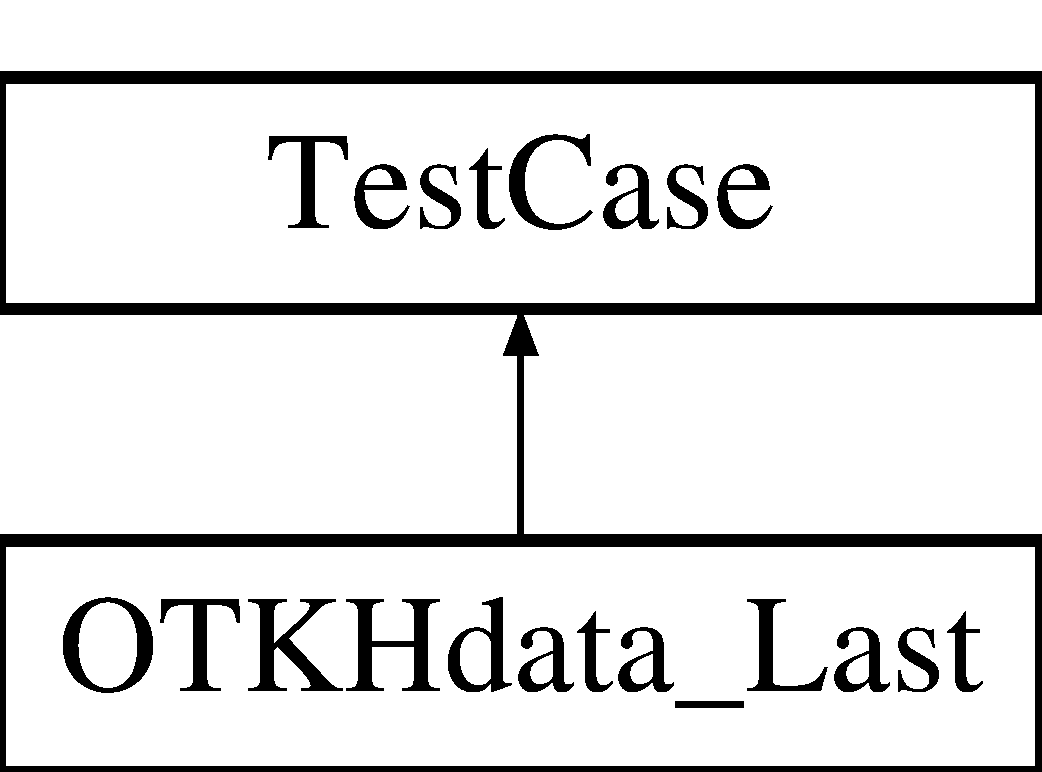
\includegraphics[height=2.000000cm]{classOTKHdata__Last}
\end{center}
\end{figure}
\subsection*{Public Member Functions}
\begin{DoxyCompactItemize}
\item 
{\bf \_\-\_\-construct} ()
\item 
{\bf prepareTest} ()
\item 
{\bf performTest} ()
\item 
{\bf cleanupTest} ()
\item 
{\bf getDetails} ()
\end{DoxyCompactItemize}
\subsection*{Private Attributes}
\begin{DoxyCompactItemize}
\item 
{\bf \$tablename}
\item 
{\bf \$details}
\end{DoxyCompactItemize}


\subsection{Detailed Description}
HData Testcase. 

This testcase dropt a database table that was used in all HData tests \begin{DoxyAuthor}{Author}
Oscar van Eijk, Oveas Functionality Provider 
\end{DoxyAuthor}
\begin{DoxyVersion}{Version}
May 23, 2011 -\/-\/ O van Eijk -\/-\/ initial version 
\end{DoxyVersion}


\subsection{Constructor \& Destructor Documentation}
\index{OTKHdata\_\-Last@{OTKHdata\_\-Last}!\_\-\_\-construct@{\_\-\_\-construct}}
\index{\_\-\_\-construct@{\_\-\_\-construct}!OTKHdata_Last@{OTKHdata\_\-Last}}
\subsubsection[{\_\-\_\-construct}]{\setlength{\rightskip}{0pt plus 5cm}OTKHdata\_\-Last::\_\-\_\-construct (
\begin{DoxyParamCaption}
{}
\end{DoxyParamCaption}
)}\label{classOTKHdata__Last_a4fc76277cb956a1e1c0e809548343ef7}
Class constuctor. All testcases must be implemented. \begin{DoxyAuthor}{Author}
Oscar van Eijk, Oveas Functionality Provider 
\end{DoxyAuthor}


Implements {\bf TestCase} \doxyref{}{p.}{interfaceTestCase_a9aac459e4d579b75426c95718790e88f}.



References OTKHdata\_\-tableName().



\subsection{Member Function Documentation}
\index{OTKHdata\_\-Last@{OTKHdata\_\-Last}!cleanupTest@{cleanupTest}}
\index{cleanupTest@{cleanupTest}!OTKHdata_Last@{OTKHdata\_\-Last}}
\subsubsection[{cleanupTest}]{\setlength{\rightskip}{0pt plus 5cm}OTKHdata\_\-Last::cleanupTest (
\begin{DoxyParamCaption}
{}
\end{DoxyParamCaption}
)}\label{classOTKHdata__Last_a32e85aa7cf89f51918ae384368e6ab4a}
Cleanup the testenvironment, e.g. drop temporary tables \begin{DoxyReturn}{Returns}
OTK\_\-RESULT\_\-SUCCESS on success, OTK\_\-RESULT\_\-NONE when this testcase needs no cleanup or an error message when failed 
\end{DoxyReturn}
\begin{DoxyAuthor}{Author}
Oscar van Eijk, Oveas Functionality Provider 
\end{DoxyAuthor}


Implements {\bf TestCase} \doxyref{}{p.}{interfaceTestCase_a71e9fd70c840ce0b535146f566e9b623}.

\index{OTKHdata\_\-Last@{OTKHdata\_\-Last}!getDetails@{getDetails}}
\index{getDetails@{getDetails}!OTKHdata_Last@{OTKHdata\_\-Last}}
\subsubsection[{getDetails}]{\setlength{\rightskip}{0pt plus 5cm}OTKHdata\_\-Last::getDetails (
\begin{DoxyParamCaption}
{}
\end{DoxyParamCaption}
)}\label{classOTKHdata__Last_ac7631fb6fe1e243712297633dc8f2327}
Gather all testdetails. During the tests, the testcase can collect all additional information in an internal datastructure, e.g. further details or explanations concerning failed tests. After finishing the testcase (and after \doxyref{cleanupTest()}{p.}{classOTKHdata__Last_a32e85aa7cf89f51918ae384368e6ab4a}), the information will be retrieved. \begin{DoxyReturn}{Returns}
Tekstblock, can contain HTML. Null and an empty textstring are allowed if no details are available. 
\end{DoxyReturn}
\begin{DoxyAuthor}{Author}
Oscar van Eijk, Oveas Functionality Provider 
\end{DoxyAuthor}


Implements {\bf TestCase} \doxyref{}{p.}{interfaceTestCase_a1abfe816e79d30871ce314dedbdf5f9d}.

\index{OTKHdata\_\-Last@{OTKHdata\_\-Last}!performTest@{performTest}}
\index{performTest@{performTest}!OTKHdata_Last@{OTKHdata\_\-Last}}
\subsubsection[{performTest}]{\setlength{\rightskip}{0pt plus 5cm}OTKHdata\_\-Last::performTest (
\begin{DoxyParamCaption}
{}
\end{DoxyParamCaption}
)}\label{classOTKHdata__Last_a9de03c5d9a332cf4ebde0be7c2a2cf79}
Perform the test(s) for this testcase. Multiple tests can be performed, each writing a single message in an internal array explaining what the result was ('step X completed succefully', an error message in case of failures etc). Additional (private) methods can be created for each step. \begin{DoxyReturn}{Returns}
A 2 dimensional array with messages for all steps that were performed in this testcase. Each step in the testcase has exactly 1 element in the array, being an array with 2 elements: first is the code as defined in \doxyref{Test result code}{p.}{group__Test__Results}, the second is an human readable message. null when the step was skipped, e.g. 
\begin{DoxyCode}
        array(
                 array(OTK_RESULT_SUCCESS, 'Step 1 completed successfully')
                ,array(OTK_RESULT_SUCCESS, 'Step 2 completed successfully')
                ,array(OTK_RESULT_FAIL, 'Step 3 failed with code XX')
                ,array(OTK_RESULT_SKIPPED, 'Step 4 could not execute because step
       3 failed')
        )
\end{DoxyCode}
 
\end{DoxyReturn}
\begin{DoxyAuthor}{Author}
Oscar van Eijk, Oveas Functionality Provider 
\end{DoxyAuthor}


Implements {\bf TestCase} \doxyref{}{p.}{interfaceTestCase_a5fcf5fd51066de41206fe02c67139c76}.



References OTKHdata\_\-getData(), and OTKHdata\_\-tableName().

\index{OTKHdata\_\-Last@{OTKHdata\_\-Last}!prepareTest@{prepareTest}}
\index{prepareTest@{prepareTest}!OTKHdata_Last@{OTKHdata\_\-Last}}
\subsubsection[{prepareTest}]{\setlength{\rightskip}{0pt plus 5cm}OTKHdata\_\-Last::prepareTest (
\begin{DoxyParamCaption}
{}
\end{DoxyParamCaption}
)}\label{classOTKHdata__Last_ad0bb7c57dac131cf01c4a1ff9df4bf47}
Prepare a testcase, e.g. create some database tables that are required for this testcase. \begin{DoxyReturn}{Returns}
OTK\_\-RESULT\_\-SUCCESS on success, OTK\_\-RESULT\_\-NONE when this testcase needs no preparation or an error message when failed 
\end{DoxyReturn}
\begin{DoxyAuthor}{Author}
Oscar van Eijk, Oveas Functionality Provider 
\end{DoxyAuthor}


Implements {\bf TestCase} \doxyref{}{p.}{interfaceTestCase_ae2fd5738550a83f15afe1cbc5365f3e8}.



\subsection{Member Data Documentation}
\index{OTKHdata\_\-Last@{OTKHdata\_\-Last}!\$details@{\$details}}
\index{\$details@{\$details}!OTKHdata_Last@{OTKHdata\_\-Last}}
\subsubsection[{\$details}]{\setlength{\rightskip}{0pt plus 5cm}OTKHdata\_\-Last::\$details\hspace{0.3cm}{\ttfamily  [private]}}\label{classOTKHdata__Last_a74e4a933ca7c77efa05bd7aa5599f855}
\index{OTKHdata\_\-Last@{OTKHdata\_\-Last}!\$tablename@{\$tablename}}
\index{\$tablename@{\$tablename}!OTKHdata_Last@{OTKHdata\_\-Last}}
\subsubsection[{\$tablename}]{\setlength{\rightskip}{0pt plus 5cm}OTKHdata\_\-Last::\$tablename\hspace{0.3cm}{\ttfamily  [private]}}\label{classOTKHdata__Last_ac9389478f14f71c1711870353b704e49}


The documentation for this class was generated from the following file:\begin{DoxyCompactItemize}
\item 
/home/oscar/projects/owl-\/php/owltestkit/testsets/hdata/{\bf case.last.php}\end{DoxyCompactItemize}

\section{OTKHdata\_\-Nodehandling Class Reference}
\label{classOTKHdata__Nodehandling}\index{OTKHdata\_\-Nodehandling@{OTKHdata\_\-Nodehandling}}


HData Node Testcase.  


Inheritance diagram for OTKHdata\_\-Nodehandling:\begin{figure}[H]
\begin{center}
\leavevmode
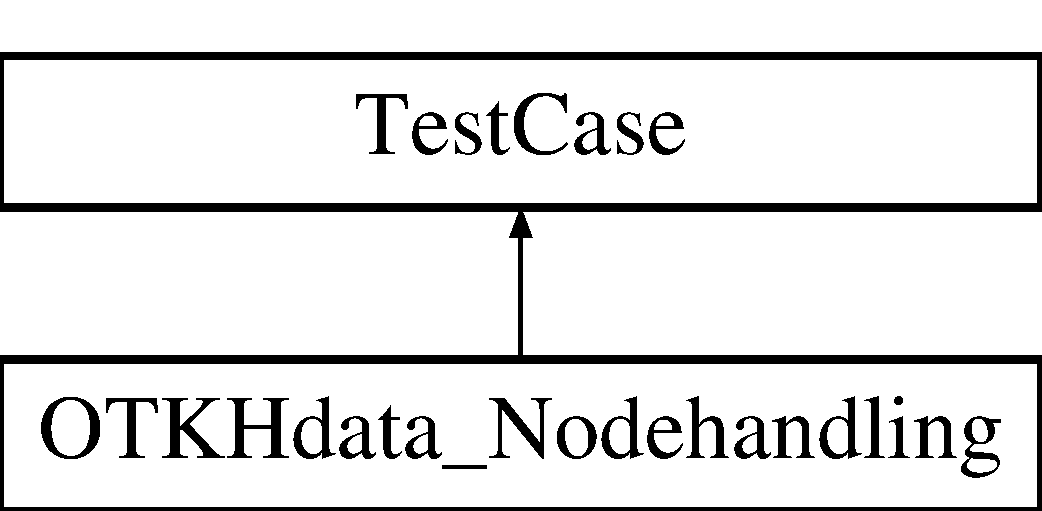
\includegraphics[height=2.000000cm]{classOTKHdata__Nodehandling}
\end{center}
\end{figure}
\subsection*{Public Member Functions}
\begin{DoxyCompactItemize}
\item 
{\bf \_\-\_\-construct} ()
\item 
{\bf prepareTest} ()
\item 
{\bf performTest} ()
\item 
{\bf cleanupTest} ()
\item 
{\bf getDetails} ()
\end{DoxyCompactItemize}
\subsection*{Private Member Functions}
\begin{DoxyCompactItemize}
\item 
{\bf checkResult} (\$retVal, \$data, \$step, \$stepDescription)
\item 
{\bf insertNodes} (\$node, \$parent)
\item 
{\bf getExpected} (\$step)
\end{DoxyCompactItemize}
\subsection*{Private Attributes}
\begin{DoxyCompactItemize}
\item 
{\bf \$hdatahandler}
\item 
{\bf \$details}
\item 
{\bf \$returnCodes}
\end{DoxyCompactItemize}


\subsection{Detailed Description}
HData Node Testcase. 

This testcase does some node handling, like inserts, move and remove \begin{DoxyAuthor}{Author}
Oscar van Eijk, Oveas Functionality Provider 
\end{DoxyAuthor}
\begin{DoxyVersion}{Version}
May 26, 2011 -\/-\/ O van Eijk -\/-\/ initial version 
\end{DoxyVersion}


\subsection{Constructor \& Destructor Documentation}
\index{OTKHdata\_\-Nodehandling@{OTKHdata\_\-Nodehandling}!\_\-\_\-construct@{\_\-\_\-construct}}
\index{\_\-\_\-construct@{\_\-\_\-construct}!OTKHdata_Nodehandling@{OTKHdata\_\-Nodehandling}}
\subsubsection[{\_\-\_\-construct}]{\setlength{\rightskip}{0pt plus 5cm}OTKHdata\_\-Nodehandling::\_\-\_\-construct (
\begin{DoxyParamCaption}
{}
\end{DoxyParamCaption}
)}\label{classOTKHdata__Nodehandling_a79e51b077cfa3a8cc736fa7e5a43ec18}
Class constuctor. All testcases must be implemented. \begin{DoxyAuthor}{Author}
Oscar van Eijk, Oveas Functionality Provider 
\end{DoxyAuthor}


Implements {\bf TestCase} \doxyref{}{p.}{interfaceTestCase_a9aac459e4d579b75426c95718790e88f}.



References OTKHdata\_\-tableName().



\subsection{Member Function Documentation}
\index{OTKHdata\_\-Nodehandling@{OTKHdata\_\-Nodehandling}!checkResult@{checkResult}}
\index{checkResult@{checkResult}!OTKHdata_Nodehandling@{OTKHdata\_\-Nodehandling}}
\subsubsection[{checkResult}]{\setlength{\rightskip}{0pt plus 5cm}OTKHdata\_\-Nodehandling::checkResult (
\begin{DoxyParamCaption}
\item[{\$}]{retVal, }
\item[{\$}]{data, }
\item[{\$}]{step, }
\item[{\$}]{stepDescription}
\end{DoxyParamCaption}
)\hspace{0.3cm}{\ttfamily  [private]}}\label{classOTKHdata__Nodehandling_ae97ed149e4e462e10aebcb6bf8f61cc1}


References OTKHelpers::compareTable(), and getExpected().



Referenced by performTest().

\index{OTKHdata\_\-Nodehandling@{OTKHdata\_\-Nodehandling}!cleanupTest@{cleanupTest}}
\index{cleanupTest@{cleanupTest}!OTKHdata_Nodehandling@{OTKHdata\_\-Nodehandling}}
\subsubsection[{cleanupTest}]{\setlength{\rightskip}{0pt plus 5cm}OTKHdata\_\-Nodehandling::cleanupTest (
\begin{DoxyParamCaption}
{}
\end{DoxyParamCaption}
)}\label{classOTKHdata__Nodehandling_adc72384179796a95e75ef4a6d0f69588}
Cleanup the testenvironment, e.g. drop temporary tables \begin{DoxyReturn}{Returns}
OTK\_\-RESULT\_\-SUCCESS on success, OTK\_\-RESULT\_\-NONE when this testcase needs no cleanup or an error message when failed 
\end{DoxyReturn}
\begin{DoxyAuthor}{Author}
Oscar van Eijk, Oveas Functionality Provider 
\end{DoxyAuthor}


Implements {\bf TestCase} \doxyref{}{p.}{interfaceTestCase_a71e9fd70c840ce0b535146f566e9b623}.

\index{OTKHdata\_\-Nodehandling@{OTKHdata\_\-Nodehandling}!getDetails@{getDetails}}
\index{getDetails@{getDetails}!OTKHdata_Nodehandling@{OTKHdata\_\-Nodehandling}}
\subsubsection[{getDetails}]{\setlength{\rightskip}{0pt plus 5cm}OTKHdata\_\-Nodehandling::getDetails (
\begin{DoxyParamCaption}
{}
\end{DoxyParamCaption}
)}\label{classOTKHdata__Nodehandling_a2dab1f57aceab77f7c2d35fbb6eaeb31}
Gather all testdetails. During the tests, the testcase can collect all additional information in an internal datastructure, e.g. further details or explanations concerning failed tests. After finishing the testcase (and after \doxyref{cleanupTest()}{p.}{classOTKHdata__Nodehandling_adc72384179796a95e75ef4a6d0f69588}), the information will be retrieved. \begin{DoxyReturn}{Returns}
Tekstblock, can contain HTML. Null and an empty textstring are allowed if no details are available. 
\end{DoxyReturn}
\begin{DoxyAuthor}{Author}
Oscar van Eijk, Oveas Functionality Provider 
\end{DoxyAuthor}


Implements {\bf TestCase} \doxyref{}{p.}{interfaceTestCase_a1abfe816e79d30871ce314dedbdf5f9d}.

\index{OTKHdata\_\-Nodehandling@{OTKHdata\_\-Nodehandling}!getExpected@{getExpected}}
\index{getExpected@{getExpected}!OTKHdata_Nodehandling@{OTKHdata\_\-Nodehandling}}
\subsubsection[{getExpected}]{\setlength{\rightskip}{0pt plus 5cm}OTKHdata\_\-Nodehandling::getExpected (
\begin{DoxyParamCaption}
\item[{\$}]{step}
\end{DoxyParamCaption}
)\hspace{0.3cm}{\ttfamily  [private]}}\label{classOTKHdata__Nodehandling_ae372d3f63601f2daef6961b18200e7d6}


Referenced by checkResult().

\index{OTKHdata\_\-Nodehandling@{OTKHdata\_\-Nodehandling}!insertNodes@{insertNodes}}
\index{insertNodes@{insertNodes}!OTKHdata_Nodehandling@{OTKHdata\_\-Nodehandling}}
\subsubsection[{insertNodes}]{\setlength{\rightskip}{0pt plus 5cm}OTKHdata\_\-Nodehandling::insertNodes (
\begin{DoxyParamCaption}
\item[{\$}]{node, }
\item[{\$}]{parent}
\end{DoxyParamCaption}
)\hspace{0.3cm}{\ttfamily  [private]}}\label{classOTKHdata__Nodehandling_a1bf44ad23c26f78240e3fbaa2bda1e71}


Referenced by performTest(), and prepareTest().

\index{OTKHdata\_\-Nodehandling@{OTKHdata\_\-Nodehandling}!performTest@{performTest}}
\index{performTest@{performTest}!OTKHdata_Nodehandling@{OTKHdata\_\-Nodehandling}}
\subsubsection[{performTest}]{\setlength{\rightskip}{0pt plus 5cm}OTKHdata\_\-Nodehandling::performTest (
\begin{DoxyParamCaption}
{}
\end{DoxyParamCaption}
)}\label{classOTKHdata__Nodehandling_a060b9a2f755669a6a229eb8aa66c0a78}
Perform the test(s) for this testcase. Multiple tests can be performed, each writing a single message in an internal array explaining what the result was ('step X completed succefully', an error message in case of failures etc). Additional (private) methods can be created for each step. \begin{DoxyReturn}{Returns}
A 2 dimensional array with messages for all steps that were performed in this testcase. Each step in the testcase has exactly 1 element in the array, being an array with 2 elements: first is the code as defined in \doxyref{Test result code}{p.}{group__Test__Results}, the second is an human readable message. null when the step was skipped, e.g. 
\begin{DoxyCode}
        array(
                 array(OTK_RESULT_SUCCESS, 'Step 1 completed successfully')
                ,array(OTK_RESULT_SUCCESS, 'Step 2 completed successfully')
                ,array(OTK_RESULT_FAIL, 'Step 3 failed with code XX')
                ,array(OTK_RESULT_SKIPPED, 'Step 4 could not execute because step
       3 failed')
        )
\end{DoxyCode}
 
\end{DoxyReturn}
\begin{DoxyAuthor}{Author}
Oscar van Eijk, Oveas Functionality Provider 
\end{DoxyAuthor}


Implements {\bf TestCase} \doxyref{}{p.}{interfaceTestCase_a5fcf5fd51066de41206fe02c67139c76}.



References checkResult(), insertNodes(), and OTKHdata\_\-getData().

\index{OTKHdata\_\-Nodehandling@{OTKHdata\_\-Nodehandling}!prepareTest@{prepareTest}}
\index{prepareTest@{prepareTest}!OTKHdata_Nodehandling@{OTKHdata\_\-Nodehandling}}
\subsubsection[{prepareTest}]{\setlength{\rightskip}{0pt plus 5cm}OTKHdata\_\-Nodehandling::prepareTest (
\begin{DoxyParamCaption}
{}
\end{DoxyParamCaption}
)}\label{classOTKHdata__Nodehandling_ad2cb9552cb84824650696dce9f59bcc7}
Prepare a testcase, e.g. create some database tables that are required for this testcase. \begin{DoxyReturn}{Returns}
OTK\_\-RESULT\_\-SUCCESS on success, OTK\_\-RESULT\_\-NONE when this testcase needs no preparation or an error message when failed 
\end{DoxyReturn}
\begin{DoxyAuthor}{Author}
Oscar van Eijk, Oveas Functionality Provider 
\end{DoxyAuthor}


Implements {\bf TestCase} \doxyref{}{p.}{interfaceTestCase_ae2fd5738550a83f15afe1cbc5365f3e8}.



References insertNodes().



\subsection{Member Data Documentation}
\index{OTKHdata\_\-Nodehandling@{OTKHdata\_\-Nodehandling}!\$details@{\$details}}
\index{\$details@{\$details}!OTKHdata_Nodehandling@{OTKHdata\_\-Nodehandling}}
\subsubsection[{\$details}]{\setlength{\rightskip}{0pt plus 5cm}OTKHdata\_\-Nodehandling::\$details\hspace{0.3cm}{\ttfamily  [private]}}\label{classOTKHdata__Nodehandling_a909901774e2de704d85fabd42ccb8934}
\index{OTKHdata\_\-Nodehandling@{OTKHdata\_\-Nodehandling}!\$hdatahandler@{\$hdatahandler}}
\index{\$hdatahandler@{\$hdatahandler}!OTKHdata_Nodehandling@{OTKHdata\_\-Nodehandling}}
\subsubsection[{\$hdatahandler}]{\setlength{\rightskip}{0pt plus 5cm}OTKHdata\_\-Nodehandling::\$hdatahandler\hspace{0.3cm}{\ttfamily  [private]}}\label{classOTKHdata__Nodehandling_a0e60a2c2585824d2a0735126b7e1d028}
\index{OTKHdata\_\-Nodehandling@{OTKHdata\_\-Nodehandling}!\$returnCodes@{\$returnCodes}}
\index{\$returnCodes@{\$returnCodes}!OTKHdata_Nodehandling@{OTKHdata\_\-Nodehandling}}
\subsubsection[{\$returnCodes}]{\setlength{\rightskip}{0pt plus 5cm}OTKHdata\_\-Nodehandling::\$returnCodes\hspace{0.3cm}{\ttfamily  [private]}}\label{classOTKHdata__Nodehandling_ab0c2b4e11e6a1d68cd6d6e6c0d2b8571}


The documentation for this class was generated from the following file:\begin{DoxyCompactItemize}
\item 
/home/oscar/projects/owl-\/php/owltestkit/testsets/hdata/{\bf case.nodehandling.php}\end{DoxyCompactItemize}

\section{OTKHelpers Class Reference}
\label{classOTKHelpers}\index{OTKHelpers@{OTKHelpers}}


\doxyref{OTK}{p.}{classOTK} Helper.  


\subsection*{Static Public Member Functions}
\begin{DoxyCompactItemize}
\item 
static {\bf compareTable} (\$expected, \$actual)
\end{DoxyCompactItemize}


\subsection{Detailed Description}
\doxyref{OTK}{p.}{classOTK} Helper. 

Abstract class with some general functions. \begin{DoxyAuthor}{Author}
Oscar van Eijk, Oveas Functionality Provider 
\end{DoxyAuthor}
\begin{DoxyVersion}{Version}
May 26, 2011 -\/-\/ O van Eijk -\/-\/ initial version 
\end{DoxyVersion}


\subsection{Member Function Documentation}
\index{OTKHelpers@{OTKHelpers}!compareTable@{compareTable}}
\index{compareTable@{compareTable}!OTKHelpers@{OTKHelpers}}
\subsubsection[{compareTable}]{\setlength{\rightskip}{0pt plus 5cm}static OTKHelpers::compareTable (
\begin{DoxyParamCaption}
\item[{\$}]{expected, }
\item[{\$}]{actual}
\end{DoxyParamCaption}
)\hspace{0.3cm}{\ttfamily  [static]}}\label{classOTKHelpers_ab5fa2fe025e87c89e51943c2ca862879}
Create a table with expected and actual testresults compared side by side 
\begin{DoxyParams}[1]{Parameters}
\mbox{\tt in}  & {\em \$expected} & The expected testresult \\
\hline
\mbox{\tt in}  & {\em \$actual} & The actual testresult \\
\hline
\end{DoxyParams}
\begin{DoxyReturn}{Returns}
HTML code 
\end{DoxyReturn}
\begin{DoxyAuthor}{Author}
Oscar van Eijk, Oveas Functionality Provider 
\end{DoxyAuthor}


Referenced by OTKHdata\_\-Nodehandling::checkResult(), OTKDbdriver\_\-First::performTest(), and OTKDbdriver\_\-Alter::performTest().



The documentation for this class was generated from the following file:\begin{DoxyCompactItemize}
\item 
/home/oscar/projects/owl-\/php/owltestkit/bo/{\bf class.otkhelpers.php}\end{DoxyCompactItemize}

\section{OTKUser Class Reference}
\label{classOTKUser}\index{OTKUser@{OTKUser}}


\doxyref{OTK}{p.}{classOTK} User.  


\subsection*{Static Public Member Functions}
\begin{DoxyCompactItemize}
\item 
static {\bf getReference} ()
\end{DoxyCompactItemize}
\subsection*{Private Member Functions}
\begin{DoxyCompactItemize}
\item 
{\bf \_\-\_\-construct} ()
\end{DoxyCompactItemize}
\subsection*{Static Private Attributes}
\begin{DoxyCompactItemize}
\item 
static {\bf \$instance}
\end{DoxyCompactItemize}


\subsection{Detailed Description}
\doxyref{OTK}{p.}{classOTK} User. 

User class. \begin{DoxyAuthor}{Author}
Oscar van Eijk, Oveas Functionality Provider 
\end{DoxyAuthor}
\begin{DoxyVersion}{Version}
May 23, 2011 -\/-\/ O van Eijk -\/-\/ initial version 
\end{DoxyVersion}


\subsection{Constructor \& Destructor Documentation}
\index{OTKUser@{OTKUser}!\_\-\_\-construct@{\_\-\_\-construct}}
\index{\_\-\_\-construct@{\_\-\_\-construct}!OTKUser@{OTKUser}}
\subsubsection[{\_\-\_\-construct}]{\setlength{\rightskip}{0pt plus 5cm}OTKUser::\_\-\_\-construct (
\begin{DoxyParamCaption}
{}
\end{DoxyParamCaption}
)\hspace{0.3cm}{\ttfamily  [private]}}\label{classOTKUser_a1cebf22203fcd29cc0f4d6beb87cb8e1}
Object constructor; private, since we want this to be a singleton here 

References \$instance.



\subsection{Member Function Documentation}
\index{OTKUser@{OTKUser}!getReference@{getReference}}
\index{getReference@{getReference}!OTKUser@{OTKUser}}
\subsubsection[{getReference}]{\setlength{\rightskip}{0pt plus 5cm}static OTKUser::getReference (
\begin{DoxyParamCaption}
{}
\end{DoxyParamCaption}
)\hspace{0.3cm}{\ttfamily  [static]}}\label{classOTKUser_a3e2f754dc345b9bd31756fbdfb7ace48}
Instantiate the singleton or return its reference 

References \$instance.



\subsection{Member Data Documentation}
\index{OTKUser@{OTKUser}!\$instance@{\$instance}}
\index{\$instance@{\$instance}!OTKUser@{OTKUser}}
\subsubsection[{\$instance}]{\setlength{\rightskip}{0pt plus 5cm}OTKUser::\$instance\hspace{0.3cm}{\ttfamily  [static, private]}}\label{classOTKUser_ab6d74502eca21716c5594f1896440135}
Self reference 

Referenced by \_\-\_\-construct(), and getReference().



The documentation for this class was generated from the following file:\begin{DoxyCompactItemize}
\item 
/home/oscar/projects/owl-\/php/owltestkit/bo/{\bf class.otkuser.php}\end{DoxyCompactItemize}

\section{TestCase Interface Reference}
\label{interfaceTestCase}\index{TestCase@{TestCase}}


Testcase.  


Inheritance diagram for TestCase:\begin{figure}[H]
\begin{center}
\leavevmode
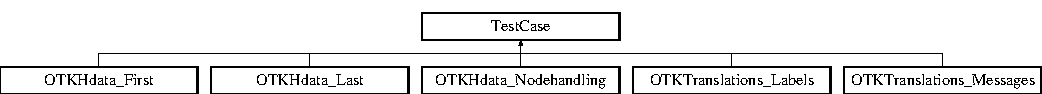
\includegraphics[height=9.000000cm]{interfaceTestCase}
\end{center}
\end{figure}
\subsection*{Public Member Functions}
\begin{DoxyCompactItemize}
\item 
{\bf \_\-\_\-construct} ()
\item 
{\bf prepareTest} ()
\item 
{\bf performTest} ()
\item 
{\bf cleanupTest} ()
\item 
{\bf getDetails} ()
\end{DoxyCompactItemize}


\subsection{Detailed Description}
Testcase. 

Interface that defines the testcase classes. Classes that implement this interface must be in a file called 'case.$<$casename$>$.php'. The classname must be 'OTK$<$Setname$>$\_\-$<$Casename$>$ where $<$casename$>$ is the name of the testcase and $<$setname$>$ the name of the testset it belongs to.

Two special casenames are reserverd: {\itshape first\/} and {\itshape last\/}, which will be the first and last testcases executed in a testset. \begin{DoxyAuthor}{Author}
Oscar van Eijk, Oveas Functionality Provider 
\end{DoxyAuthor}
\begin{DoxyVersion}{Version}
May 19, 2011 -\/-\/ O van Eijk -\/-\/ initial version 
\end{DoxyVersion}


\subsection{Constructor \& Destructor Documentation}
\index{TestCase@{TestCase}!\_\-\_\-construct@{\_\-\_\-construct}}
\index{\_\-\_\-construct@{\_\-\_\-construct}!TestCase@{TestCase}}
\subsubsection[{\_\-\_\-construct}]{\setlength{\rightskip}{0pt plus 5cm}TestCase::\_\-\_\-construct (
\begin{DoxyParamCaption}
{}
\end{DoxyParamCaption}
)}\label{interfaceTestCase_a9aac459e4d579b75426c95718790e88f}
Class constuctor. All testcases must be implemented. \begin{DoxyAuthor}{Author}
Oscar van Eijk, Oveas Functionality Provider 
\end{DoxyAuthor}


Implemented in {\bf OTKDbdriver\_\-Alter} \doxyref{}{p.}{classOTKDbdriver__Alter_a07bf0954617a751361ae8d5b2f9c4232}, {\bf OTKDbdriver\_\-First} \doxyref{}{p.}{classOTKDbdriver__First_a484746d0a22a3f94a0db2e55bf8c9bbe}, {\bf OTKDbdriver\_\-Last} \doxyref{}{p.}{classOTKDbdriver__Last_a3fa38c164dff1e89b07992031d2395bc}, {\bf OTKHdata\_\-First} \doxyref{}{p.}{classOTKHdata__First_a5f565719287cedfca6c95b79ca0eae7f}, {\bf OTKHdata\_\-Last} \doxyref{}{p.}{classOTKHdata__Last_a4fc76277cb956a1e1c0e809548343ef7}, {\bf OTKHdata\_\-Nodehandling} \doxyref{}{p.}{classOTKHdata__Nodehandling_a79e51b077cfa3a8cc736fa7e5a43ec18}, {\bf OTKTranslations\_\-Labels} \doxyref{}{p.}{classOTKTranslations__Labels_afd405b061305a8eff86234bbf1816cc3}, and {\bf OTKTranslations\_\-Messages} \doxyref{}{p.}{classOTKTranslations__Messages_a6462f7b6b0ea3720392a448a1dacfc42}.



\subsection{Member Function Documentation}
\index{TestCase@{TestCase}!cleanupTest@{cleanupTest}}
\index{cleanupTest@{cleanupTest}!TestCase@{TestCase}}
\subsubsection[{cleanupTest}]{\setlength{\rightskip}{0pt plus 5cm}TestCase::cleanupTest (
\begin{DoxyParamCaption}
{}
\end{DoxyParamCaption}
)}\label{interfaceTestCase_a71e9fd70c840ce0b535146f566e9b623}
Cleanup the testenvironment, e.g. drop temporary tables \begin{DoxyReturn}{Returns}
OTK\_\-RESULT\_\-SUCCESS on success, OTK\_\-RESULT\_\-NONE when this testcase needs no cleanup or an error message when failed 
\end{DoxyReturn}
\begin{DoxyAuthor}{Author}
Oscar van Eijk, Oveas Functionality Provider 
\end{DoxyAuthor}


Implemented in {\bf OTKDbdriver\_\-Alter} \doxyref{}{p.}{classOTKDbdriver__Alter_a134d4dfba456ab717d11d3b59374e822}, {\bf OTKDbdriver\_\-First} \doxyref{}{p.}{classOTKDbdriver__First_a696654ed37e17d9c2a7a5f1678a5b2a8}, {\bf OTKDbdriver\_\-Last} \doxyref{}{p.}{classOTKDbdriver__Last_a3a47ada2c14fc08421ac73fffcd06a8d}, {\bf OTKHdata\_\-First} \doxyref{}{p.}{classOTKHdata__First_aeedd9ae405d5e5e6f2e37b597b2e798e}, {\bf OTKHdata\_\-Last} \doxyref{}{p.}{classOTKHdata__Last_a32e85aa7cf89f51918ae384368e6ab4a}, {\bf OTKHdata\_\-Nodehandling} \doxyref{}{p.}{classOTKHdata__Nodehandling_adc72384179796a95e75ef4a6d0f69588}, {\bf OTKTranslations\_\-Labels} \doxyref{}{p.}{classOTKTranslations__Labels_ac691c68fa8a35d6e5685fd04b1d14a5b}, and {\bf OTKTranslations\_\-Messages} \doxyref{}{p.}{classOTKTranslations__Messages_a3cf1534e4d2a4294c95562ff62ccf367}.

\index{TestCase@{TestCase}!getDetails@{getDetails}}
\index{getDetails@{getDetails}!TestCase@{TestCase}}
\subsubsection[{getDetails}]{\setlength{\rightskip}{0pt plus 5cm}TestCase::getDetails (
\begin{DoxyParamCaption}
{}
\end{DoxyParamCaption}
)}\label{interfaceTestCase_a1abfe816e79d30871ce314dedbdf5f9d}
Gather all testdetails. During the tests, the testcase can collect all additional information in an internal datastructure, e.g. further details or explanations concerning failed tests. After finishing the testcase (and after \doxyref{cleanupTest()}{p.}{interfaceTestCase_a71e9fd70c840ce0b535146f566e9b623}), the information will be retrieved. \begin{DoxyReturn}{Returns}
Tekstblock, can contain HTML. Null and an empty textstring are allowed if no details are available. 
\end{DoxyReturn}
\begin{DoxyAuthor}{Author}
Oscar van Eijk, Oveas Functionality Provider 
\end{DoxyAuthor}


Implemented in {\bf OTKDbdriver\_\-Alter} \doxyref{}{p.}{classOTKDbdriver__Alter_a74228b8f51b01c806454c163645d7ebb}, {\bf OTKDbdriver\_\-First} \doxyref{}{p.}{classOTKDbdriver__First_a0d2147f25ab91b9451dbfc3645dec720}, {\bf OTKDbdriver\_\-Last} \doxyref{}{p.}{classOTKDbdriver__Last_a6c045ef32dd6f50ec9cd2a38086ee254}, {\bf OTKHdata\_\-First} \doxyref{}{p.}{classOTKHdata__First_a7da202076d69c882a2b0cbed36556c26}, {\bf OTKHdata\_\-Last} \doxyref{}{p.}{classOTKHdata__Last_ac7631fb6fe1e243712297633dc8f2327}, {\bf OTKHdata\_\-Nodehandling} \doxyref{}{p.}{classOTKHdata__Nodehandling_a2dab1f57aceab77f7c2d35fbb6eaeb31}, {\bf OTKTranslations\_\-Labels} \doxyref{}{p.}{classOTKTranslations__Labels_ae4a004a59e68a4a9321d56d1a594aea3}, and {\bf OTKTranslations\_\-Messages} \doxyref{}{p.}{classOTKTranslations__Messages_a74e7ec342bfb1c0130921a1d5f282dbf}.

\index{TestCase@{TestCase}!performTest@{performTest}}
\index{performTest@{performTest}!TestCase@{TestCase}}
\subsubsection[{performTest}]{\setlength{\rightskip}{0pt plus 5cm}TestCase::performTest (
\begin{DoxyParamCaption}
{}
\end{DoxyParamCaption}
)}\label{interfaceTestCase_a5fcf5fd51066de41206fe02c67139c76}
Perform the test(s) for this testcase. Multiple tests can be performed, each writing a single message in an internal array explaining what the result was ('step X completed succefully', an error message in case of failures etc). Additional (private) methods can be created for each step. \begin{DoxyReturn}{Returns}
A 2 dimensional array with messages for all steps that were performed in this testcase. Each step in the testcase has exactly 1 element in the array, being an array with 2 elements: first is the code as defined in \doxyref{Test result code}{p.}{group__Test__Results}, the second is an human readable message. null when the step was skipped, e.g. 
\begin{DoxyCode}
        array(
                 array(OTK_RESULT_SUCCESS, 'Step 1 completed successfully')
                ,array(OTK_RESULT_SUCCESS, 'Step 2 completed successfully')
                ,array(OTK_RESULT_FAIL, 'Step 3 failed with code XX')
                ,array(OTK_RESULT_SKIPPED, 'Step 4 could not execute because step
       3 failed')
        )
\end{DoxyCode}
 
\end{DoxyReturn}
\begin{DoxyAuthor}{Author}
Oscar van Eijk, Oveas Functionality Provider 
\end{DoxyAuthor}


Implemented in {\bf OTKDbdriver\_\-Alter} \doxyref{}{p.}{classOTKDbdriver__Alter_a180a9fc45b42aa18cab916467c499c39}, {\bf OTKDbdriver\_\-First} \doxyref{}{p.}{classOTKDbdriver__First_a8e4971170bc40db4ec123f81059189a6}, {\bf OTKDbdriver\_\-Last} \doxyref{}{p.}{classOTKDbdriver__Last_a345dd22c2758c229f304f6a7a9d35d0d}, {\bf OTKHdata\_\-First} \doxyref{}{p.}{classOTKHdata__First_a5fc1c37ab0f64861e37688df17922a00}, {\bf OTKHdata\_\-Last} \doxyref{}{p.}{classOTKHdata__Last_a9de03c5d9a332cf4ebde0be7c2a2cf79}, {\bf OTKHdata\_\-Nodehandling} \doxyref{}{p.}{classOTKHdata__Nodehandling_a060b9a2f755669a6a229eb8aa66c0a78}, {\bf OTKTranslations\_\-Labels} \doxyref{}{p.}{classOTKTranslations__Labels_abf394fe332bbdc9dc38b28d33b88637c}, and {\bf OTKTranslations\_\-Messages} \doxyref{}{p.}{classOTKTranslations__Messages_a2b2de47926411b5d79aa4daf5d36570b}.

\index{TestCase@{TestCase}!prepareTest@{prepareTest}}
\index{prepareTest@{prepareTest}!TestCase@{TestCase}}
\subsubsection[{prepareTest}]{\setlength{\rightskip}{0pt plus 5cm}TestCase::prepareTest (
\begin{DoxyParamCaption}
{}
\end{DoxyParamCaption}
)}\label{interfaceTestCase_ae2fd5738550a83f15afe1cbc5365f3e8}
Prepare a testcase, e.g. create some database tables that are required for this testcase. \begin{DoxyReturn}{Returns}
OTK\_\-RESULT\_\-SUCCESS on success, OTK\_\-RESULT\_\-NONE when this testcase needs no preparation or an error message when failed 
\end{DoxyReturn}
\begin{DoxyAuthor}{Author}
Oscar van Eijk, Oveas Functionality Provider 
\end{DoxyAuthor}


Implemented in {\bf OTKDbdriver\_\-Alter} \doxyref{}{p.}{classOTKDbdriver__Alter_a700459f4ab0ecdb58b2f6d7fd7c58f3f}, {\bf OTKDbdriver\_\-First} \doxyref{}{p.}{classOTKDbdriver__First_a190b57fdaf6e35c32197da51784ae86f}, {\bf OTKDbdriver\_\-Last} \doxyref{}{p.}{classOTKDbdriver__Last_a9e0062f9c4d370143d815f03fa9c74cd}, {\bf OTKHdata\_\-First} \doxyref{}{p.}{classOTKHdata__First_afb8f48a3f84fda934fc4005032bb3547}, {\bf OTKHdata\_\-Last} \doxyref{}{p.}{classOTKHdata__Last_ad0bb7c57dac131cf01c4a1ff9df4bf47}, {\bf OTKHdata\_\-Nodehandling} \doxyref{}{p.}{classOTKHdata__Nodehandling_ad2cb9552cb84824650696dce9f59bcc7}, {\bf OTKTranslations\_\-Labels} \doxyref{}{p.}{classOTKTranslations__Labels_a0ff19826602fd6503ddc25fdf00ff034}, and {\bf OTKTranslations\_\-Messages} \doxyref{}{p.}{classOTKTranslations__Messages_a8695218421416f2836f768df5213a17f}.



The documentation for this interface was generated from the following file:\begin{DoxyCompactItemize}
\item 
/home/oscar/projects/owl-\/php/owltestkit/bo/{\bf class.testcase.php}\end{DoxyCompactItemize}

\section{TestKit Class Reference}
\label{classTestKit}\index{TestKit@{TestKit}}


Testset loader.  


\subsection*{Public Member Functions}
\begin{DoxyCompactItemize}
\item 
{\bf getTestSets} ()
\item 
{\bf performTests} (\$testSet)
\end{DoxyCompactItemize}
\subsection*{Static Public Member Functions}
\begin{DoxyCompactItemize}
\item 
static {\bf getInstance} ()
\end{DoxyCompactItemize}
\subsection*{Private Member Functions}
\begin{DoxyCompactItemize}
\item 
{\bf \_\-\_\-construct} ()
\item 
{\bf loadTestSet} (\$name)
\item 
{\bf getClassName} (\$setName)
\end{DoxyCompactItemize}
\subsection*{Private Attributes}
\begin{DoxyCompactItemize}
\item 
{\bf \$sets}
\end{DoxyCompactItemize}
\subsection*{Static Private Attributes}
\begin{DoxyCompactItemize}
\item 
static {\bf \$instance}
\end{DoxyCompactItemize}


\subsection{Detailed Description}
Testset loader. 

Singleton class that loads all testsets \begin{DoxyAuthor}{Author}
Oscar van Eijk, Oveas Functionality Provider 
\end{DoxyAuthor}
\begin{DoxyVersion}{Version}
May 19, 2011 -\/-\/ O van Eijk -\/-\/ initial version 
\end{DoxyVersion}


\subsection{Constructor \& Destructor Documentation}
\index{TestKit@{TestKit}!\_\-\_\-construct@{\_\-\_\-construct}}
\index{\_\-\_\-construct@{\_\-\_\-construct}!TestKit@{TestKit}}
\subsubsection[{\_\-\_\-construct}]{\setlength{\rightskip}{0pt plus 5cm}TestKit::\_\-\_\-construct (
\begin{DoxyParamCaption}
{}
\end{DoxyParamCaption}
)\hspace{0.3cm}{\ttfamily  [private]}}\label{classTestKit_a8b1c19958ea1fef97afb0ef02838f83e}
Class constructor; scan the testsets directory for subdirectories that can contain testsets, and load all testset -\/ classfiles that have been found. \begin{DoxyAuthor}{Author}
Oscar van Eijk, Oveas Functionality Provider 
\end{DoxyAuthor}


References loadTestSet().



\subsection{Member Function Documentation}
\index{TestKit@{TestKit}!getClassName@{getClassName}}
\index{getClassName@{getClassName}!TestKit@{TestKit}}
\subsubsection[{getClassName}]{\setlength{\rightskip}{0pt plus 5cm}TestKit::getClassName (
\begin{DoxyParamCaption}
\item[{\$}]{setName}
\end{DoxyParamCaption}
)\hspace{0.3cm}{\ttfamily  [private]}}\label{classTestKit_a1fed7be3ce14ebafe682244b3ca017a5}
Translate the setname (taken from the directory name) into a classname in the required format 
\begin{DoxyParams}[1]{Parameters}
\mbox{\tt in}  & {\em \$setName} & Name of the set and directory \\
\hline
\end{DoxyParams}
\begin{DoxyReturn}{Returns}
Classname 
\end{DoxyReturn}
\begin{DoxyAuthor}{Author}
Oscar van Eijk, Oveas Functionality Provider 
\end{DoxyAuthor}


Referenced by loadTestSet(), and performTests().

\index{TestKit@{TestKit}!getInstance@{getInstance}}
\index{getInstance@{getInstance}!TestKit@{TestKit}}
\subsubsection[{getInstance}]{\setlength{\rightskip}{0pt plus 5cm}static TestKit::getInstance (
\begin{DoxyParamCaption}
{}
\end{DoxyParamCaption}
)\hspace{0.3cm}{\ttfamily  [static]}}\label{classTestKit_ab2fdf74a60ab20ebcc1ed7a087951355}
Return a reference to my implementation. If necessary, create that implementation first. \begin{DoxyReturn}{Returns}
Object instance ID 
\end{DoxyReturn}
\begin{DoxyAuthor}{Author}
Oscar van Eijk, Oveas Functionality Provider 
\end{DoxyAuthor}


References \$instance.

\index{TestKit@{TestKit}!getTestSets@{getTestSets}}
\index{getTestSets@{getTestSets}!TestKit@{TestKit}}
\subsubsection[{getTestSets}]{\setlength{\rightskip}{0pt plus 5cm}TestKit::getTestSets (
\begin{DoxyParamCaption}
{}
\end{DoxyParamCaption}
)}\label{classTestKit_a831800f63e9299bfbbe46ed3a2f19480}
Return the available tests \begin{DoxyReturn}{Returns}
Testsets as an indexed array in the format (name =$>$ description) 
\end{DoxyReturn}
\begin{DoxyAuthor}{Author}
Oscar van Eijk, Oveas Functionality Provider 
\end{DoxyAuthor}
\index{TestKit@{TestKit}!loadTestSet@{loadTestSet}}
\index{loadTestSet@{loadTestSet}!TestKit@{TestKit}}
\subsubsection[{loadTestSet}]{\setlength{\rightskip}{0pt plus 5cm}TestKit::loadTestSet (
\begin{DoxyParamCaption}
\item[{\$}]{name}
\end{DoxyParamCaption}
)\hspace{0.3cm}{\ttfamily  [private]}}\label{classTestKit_a2dc6a2ac4e931bb8b9a0bd909e6f5233}
Check if a directory contains a testset. If so, load the classfile and add the testset name and description to the internal array. 
\begin{DoxyParams}[1]{Parameters}
\mbox{\tt in}  & {\em \$name} & Name of the directory to check \\
\hline
\end{DoxyParams}
\begin{DoxyReturn}{Returns}
null if the directory contains no valid testset, true when successfully loaded, false on errors. 
\end{DoxyReturn}
\begin{DoxyAuthor}{Author}
Oscar van Eijk, Oveas Functionality Provider 
\end{DoxyAuthor}


References getClassName().



Referenced by \_\-\_\-construct().

\index{TestKit@{TestKit}!performTests@{performTests}}
\index{performTests@{performTests}!TestKit@{TestKit}}
\subsubsection[{performTests}]{\setlength{\rightskip}{0pt plus 5cm}TestKit::performTests (
\begin{DoxyParamCaption}
\item[{\$}]{testSet}
\end{DoxyParamCaption}
)}\label{classTestKit_adf785b6be468866f96c0b627d7a1e868}
Perform the testcases of a given testset 
\begin{DoxyParams}[1]{Parameters}
\mbox{\tt in}  & {\em \$testSet} & Testset to perform \\
\hline
\end{DoxyParams}
\begin{DoxyAuthor}{Author}
Oscar van Eijk, Oveas Functionality Provider 
\end{DoxyAuthor}


References getClassName().



\subsection{Member Data Documentation}
\index{TestKit@{TestKit}!\$instance@{\$instance}}
\index{\$instance@{\$instance}!TestKit@{TestKit}}
\subsubsection[{\$instance}]{\setlength{\rightskip}{0pt plus 5cm}TestKit::\$instance\hspace{0.3cm}{\ttfamily  [static, private]}}\label{classTestKit_a3d2f4e29a9b1aba210a38cf8d1826adc}
Self reference 

Referenced by getInstance().

\index{TestKit@{TestKit}!\$sets@{\$sets}}
\index{\$sets@{\$sets}!TestKit@{TestKit}}
\subsubsection[{\$sets}]{\setlength{\rightskip}{0pt plus 5cm}TestKit::\$sets\hspace{0.3cm}{\ttfamily  [private]}}\label{classTestKit_af6d52c4544fdaa0c717aefeafcd5688e}
Indexed array with all testsets and their descriptions 

The documentation for this class was generated from the following file:\begin{DoxyCompactItemize}
\item 
/home/oscar/projects/owl-\/php/owltestkit/so/{\bf class.testkit.php}\end{DoxyCompactItemize}

\section{TestresultsArea Class Reference}
\label{classTestresultsArea}\index{TestresultsArea@{TestresultsArea}}


List knowledge.  


\subsection*{Public Member Functions}
\begin{DoxyCompactItemize}
\item 
{\bf loadArea} (\$arg=null)
\end{DoxyCompactItemize}
\subsection*{Private Attributes}
\begin{DoxyCompactItemize}
\item 
{\bf \$testKit}
\end{DoxyCompactItemize}


\subsection{Detailed Description}
List knowledge. 

Setup the contentarea showing all testresults \begin{DoxyAuthor}{Author}
Oscar van Eijk, Oveas Functionality Provider 
\end{DoxyAuthor}
\begin{DoxyVersion}{Version}
May 18, 2011 -\/-\/ O van Eijk -\/-\/ initial version 
\end{DoxyVersion}


\subsection{Member Function Documentation}
\index{TestresultsArea@{TestresultsArea}!loadArea@{loadArea}}
\index{loadArea@{loadArea}!TestresultsArea@{TestresultsArea}}
\subsubsection[{loadArea}]{\setlength{\rightskip}{0pt plus 5cm}TestresultsArea::loadArea (
\begin{DoxyParamCaption}
\item[{\$}]{arg = {\ttfamily null}}
\end{DoxyParamCaption}
)}\label{classTestresultsArea_a3b56537970c387e0e37700eb670c0dd3}
Show all results for a given testset 
\begin{DoxyParams}[1]{Parameters}
\mbox{\tt in}  & {\em \$arg} & Array with all results \\
\hline
\end{DoxyParams}


\subsection{Member Data Documentation}
\index{TestresultsArea@{TestresultsArea}!\$testKit@{\$testKit}}
\index{\$testKit@{\$testKit}!TestresultsArea@{TestresultsArea}}
\subsubsection[{\$testKit}]{\setlength{\rightskip}{0pt plus 5cm}TestresultsArea::\$testKit\hspace{0.3cm}{\ttfamily  [private]}}\label{classTestresultsArea_a44b10285c3f21c9bfc5cbf8b7deca72c}


The documentation for this class was generated from the following file:\begin{DoxyCompactItemize}
\item 
/home/oscar/projects/owl-\/php/owltestkit/ui/{\bf testresults.php}\end{DoxyCompactItemize}

\section{TestSet Class Reference}
\label{classTestSet}\index{TestSet@{TestSet}}


Testset.  


Inheritance diagram for TestSet:\begin{figure}[H]
\begin{center}
\leavevmode
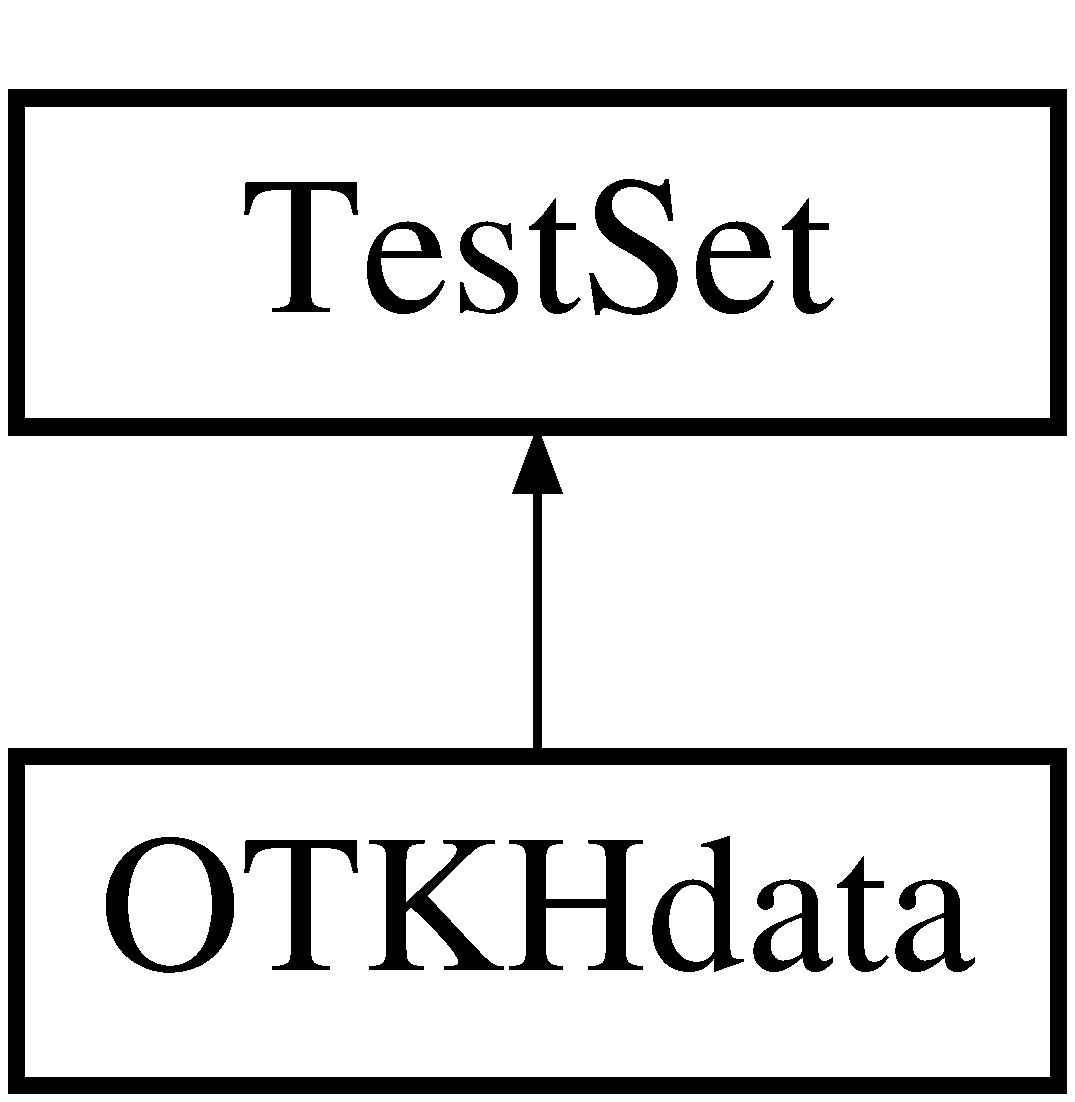
\includegraphics[height=2.000000cm]{classTestSet}
\end{center}
\end{figure}
\subsection*{Public Member Functions}
\begin{DoxyCompactItemize}
\item 
{\bf \_\-\_\-construct} ()
\item 
{\bf loadTestcases} (\$location)
\item 
{\bf performTests} ()
\end{DoxyCompactItemize}
\subsection*{Static Public Member Functions}
\begin{DoxyCompactItemize}
\item 
static {\bf getDescription} ()
\end{DoxyCompactItemize}
\subsection*{Private Member Functions}
\begin{DoxyCompactItemize}
\item 
{\bf doTest} (\$name, \$file)
\item 
{\bf showTestResults} ()
\end{DoxyCompactItemize}
\subsection*{Private Attributes}
\begin{DoxyCompactItemize}
\item 
{\bf \$setName}
\item 
{\bf \$helper}
\item 
{\bf \$testCases}
\item 
{\bf \$details}
\item 
{\bf \$testResults}
\item 
{\bf \$errors}
\item 
{\bf \$warnings}
\item 
{\bf \$succeeded}
\item 
{\bf \$skipped}
\end{DoxyCompactItemize}


\subsection{Detailed Description}
Testset. 

Baseclass that defines the testsets. Classes that derive from this baseclass must have the name {\itshape \doxyref{OTK}{p.}{classOTK}$<$Location$>$\/}, where 'location' is the name of the subdirectory in OTK\_\-TESTSETS. The filename must be {\itshape testset.php\/}.

The classes only need to reimplement the static \doxyref{getDescription()}{p.}{classTestSet_ab5b54e632b3de37daaceea3d922658bf} method, all other required methods are in this baseclass.

The class collects all files belonging to a testset that contain testcases and helper functions. All files must be in the same directory as {\itshape testset.php\/}.

Files that contain testcases must have the name {\itshape case.$<$name$>$.php\/}. Refer to the interface \doxyref{TestCase}{p.}{interfaceTestCase} for more information.

Optionally, testset directories can contain a file with the name {\itshape helper.php\/}. This can be a file containing one or more classes or functions. That file will be included but not called; it is up to the testcases to make the proper calls to these files. In order prevent duplicate class or function names, it is a good practice to include the name of the testset in in all names. \begin{DoxyAuthor}{Author}
Oscar van Eijk, Oveas Functionality Provider 
\end{DoxyAuthor}
\begin{DoxyVersion}{Version}
May 19, 2011 -\/-\/ O van Eijk -\/-\/ initial version 
\end{DoxyVersion}


\subsection{Constructor \& Destructor Documentation}
\index{TestSet@{TestSet}!\_\-\_\-construct@{\_\-\_\-construct}}
\index{\_\-\_\-construct@{\_\-\_\-construct}!TestSet@{TestSet}}
\subsubsection[{\_\-\_\-construct}]{\setlength{\rightskip}{0pt plus 5cm}TestSet::\_\-\_\-construct (
\begin{DoxyParamCaption}
{}
\end{DoxyParamCaption}
)}\label{classTestSet_a668ef2c881ce68d460d10ac3fb0791ef}
Class constructor \begin{DoxyAuthor}{Author}
Oscar van Eijk, Oveas Functionality Provider 
\end{DoxyAuthor}


\subsection{Member Function Documentation}
\index{TestSet@{TestSet}!doTest@{doTest}}
\index{doTest@{doTest}!TestSet@{TestSet}}
\subsubsection[{doTest}]{\setlength{\rightskip}{0pt plus 5cm}TestSet::doTest (
\begin{DoxyParamCaption}
\item[{\$}]{name, }
\item[{\$}]{file}
\end{DoxyParamCaption}
)\hspace{0.3cm}{\ttfamily  [private]}}\label{classTestSet_acd364b694ebba50bd71260398314369e}
Execute a single testcase 
\begin{DoxyParams}[1]{Parameters}
\mbox{\tt in}  & {\em \$name} & Name of the testcase \\
\hline
\mbox{\tt in}  & {\em \$file} & Full path to the testcase file \\
\hline
\end{DoxyParams}
\begin{DoxyAuthor}{Author}
Oscar van Eijk, Oveas Functionality Provider 
\end{DoxyAuthor}


Referenced by performTests().

\index{TestSet@{TestSet}!getDescription@{getDescription}}
\index{getDescription@{getDescription}!TestSet@{TestSet}}
\subsubsection[{getDescription}]{\setlength{\rightskip}{0pt plus 5cm}static TestSet::getDescription (
\begin{DoxyParamCaption}
{}
\end{DoxyParamCaption}
)\hspace{0.3cm}{\ttfamily  [static]}}\label{classTestSet_ab5b54e632b3de37daaceea3d922658bf}
This is the only required method that should be implemented by Testset classes; it shows a description of the testset. \begin{DoxyNote}{Note}
This method must be reimplemented, but it cannot be declared abstract since it is a static method. Since it is static, it does belong to the class itself, meaning this method here will never be called; it is included just for documentation purposes. 
\end{DoxyNote}
\begin{DoxyReturn}{Returns}
A textstring (HTML allowed) describing the testset 
\end{DoxyReturn}
\begin{DoxyAuthor}{Author}
Oscar van Eijk, Oveas Functionality Provider 
\end{DoxyAuthor}


Reimplemented in {\bf OTKDbdriver} \doxyref{}{p.}{classOTKDbdriver_aafd08a2669da0952fcc12738b54423b5}, {\bf OTKHdata} \doxyref{}{p.}{classOTKHdata_a483426fa42c2f7c1718b207b03046a0f}, and {\bf OTKTranslations} \doxyref{}{p.}{classOTKTranslations_a79ba280f3d7cd932c872e80d87bb9d93}.

\index{TestSet@{TestSet}!loadTestcases@{loadTestcases}}
\index{loadTestcases@{loadTestcases}!TestSet@{TestSet}}
\subsubsection[{loadTestcases}]{\setlength{\rightskip}{0pt plus 5cm}TestSet::loadTestcases (
\begin{DoxyParamCaption}
\item[{\$}]{location}
\end{DoxyParamCaption}
)}\label{classTestSet_a81918b70986d21e7406d9dbec9e3d801}
Scan the testset directory for all files holeing either testcases ({\itshape case.$<$name$>$.php\/}) or helper functions or class ({\itshape helper.php\/}). 
\begin{DoxyParams}[1]{Parameters}
\mbox{\tt in}  & {\em \$location} & Directory to scan \\
\hline
\end{DoxyParams}
\begin{DoxyAuthor}{Author}
Oscar van Eijk, Oveas Functionality Provider 
\end{DoxyAuthor}
\index{TestSet@{TestSet}!performTests@{performTests}}
\index{performTests@{performTests}!TestSet@{TestSet}}
\subsubsection[{performTests}]{\setlength{\rightskip}{0pt plus 5cm}TestSet::performTests (
\begin{DoxyParamCaption}
{}
\end{DoxyParamCaption}
)}\label{classTestSet_a1885d85f93b94cff6a04a038a676c63e}
Go through all selected testcases and execute them \begin{DoxyAuthor}{Author}
Oscar van Eijk, Oveas Functionality Provider 
\end{DoxyAuthor}


References doTest(), and showTestResults().

\index{TestSet@{TestSet}!showTestResults@{showTestResults}}
\index{showTestResults@{showTestResults}!TestSet@{TestSet}}
\subsubsection[{showTestResults}]{\setlength{\rightskip}{0pt plus 5cm}TestSet::showTestResults (
\begin{DoxyParamCaption}
{}
\end{DoxyParamCaption}
)\hspace{0.3cm}{\ttfamily  [private]}}\label{classTestSet_a5ded5b652032e19ae4f638f6fe63a3fa}
Create the contentarea to display the results. To make sure we don't need to wait until all tests completed, the output is echoed immediatly. \begin{DoxyAuthor}{Author}
Oscar van Eijk, Oveas Functionality Provider 
\end{DoxyAuthor}


Referenced by performTests().



\subsection{Member Data Documentation}
\index{TestSet@{TestSet}!\$details@{\$details}}
\index{\$details@{\$details}!TestSet@{TestSet}}
\subsubsection[{\$details}]{\setlength{\rightskip}{0pt plus 5cm}TestSet::\$details\hspace{0.3cm}{\ttfamily  [private]}}\label{classTestSet_aca0a0b885b900339ebd965bbaeef33e6}
Details description of the testresults \index{TestSet@{TestSet}!\$errors@{\$errors}}
\index{\$errors@{\$errors}!TestSet@{TestSet}}
\subsubsection[{\$errors}]{\setlength{\rightskip}{0pt plus 5cm}TestSet::\$errors\hspace{0.3cm}{\ttfamily  [private]}}\label{classTestSet_a0746e54ef54b321e6a785ac115a9b8cb}
Total number of teststeps that ended in an error \index{TestSet@{TestSet}!\$helper@{\$helper}}
\index{\$helper@{\$helper}!TestSet@{TestSet}}
\subsubsection[{\$helper}]{\setlength{\rightskip}{0pt plus 5cm}TestSet::\$helper\hspace{0.3cm}{\ttfamily  [private]}}\label{classTestSet_af924384ac634f0444aa4f6ac1776fe50}
Full path to the helper file ('helper.php') if this set contains one \index{TestSet@{TestSet}!\$setName@{\$setName}}
\index{\$setName@{\$setName}!TestSet@{TestSet}}
\subsubsection[{\$setName}]{\setlength{\rightskip}{0pt plus 5cm}TestSet::\$setName\hspace{0.3cm}{\ttfamily  [private]}}\label{classTestSet_a1f1174f715346d8a39e67970f700a677}
Name of the testset. It will be taken from the classname (without the leading 'OTK') \index{TestSet@{TestSet}!\$skipped@{\$skipped}}
\index{\$skipped@{\$skipped}!TestSet@{TestSet}}
\subsubsection[{\$skipped}]{\setlength{\rightskip}{0pt plus 5cm}TestSet::\$skipped\hspace{0.3cm}{\ttfamily  [private]}}\label{classTestSet_acd7b0a8534a6841a0bce26fee6cc769c}
Total number of teststeps that have been skipped \index{TestSet@{TestSet}!\$succeeded@{\$succeeded}}
\index{\$succeeded@{\$succeeded}!TestSet@{TestSet}}
\subsubsection[{\$succeeded}]{\setlength{\rightskip}{0pt plus 5cm}TestSet::\$succeeded\hspace{0.3cm}{\ttfamily  [private]}}\label{classTestSet_a0b8f595a3c60d672e7dac630cf09132b}
Total number of teststeps that completed successfull \index{TestSet@{TestSet}!\$testCases@{\$testCases}}
\index{\$testCases@{\$testCases}!TestSet@{TestSet}}
\subsubsection[{\$testCases}]{\setlength{\rightskip}{0pt plus 5cm}TestSet::\$testCases\hspace{0.3cm}{\ttfamily  [private]}}\label{classTestSet_abe27f3fb31dd64d909963914412ac866}
Indexed array holding all testcases found in this set \index{TestSet@{TestSet}!\$testResults@{\$testResults}}
\index{\$testResults@{\$testResults}!TestSet@{TestSet}}
\subsubsection[{\$testResults}]{\setlength{\rightskip}{0pt plus 5cm}TestSet::\$testResults\hspace{0.3cm}{\ttfamily  [private]}}\label{classTestSet_a9841ef8a6c8ce307f780bce7c2a30bb0}
Indexed array with the results of all steps per testcase \index{TestSet@{TestSet}!\$warnings@{\$warnings}}
\index{\$warnings@{\$warnings}!TestSet@{TestSet}}
\subsubsection[{\$warnings}]{\setlength{\rightskip}{0pt plus 5cm}TestSet::\$warnings\hspace{0.3cm}{\ttfamily  [private]}}\label{classTestSet_a805a35b038909669a923c67b97f76082}
Total number of teststeps that ended with a warning 

The documentation for this class was generated from the following file:\begin{DoxyCompactItemize}
\item 
/home/oscar/projects/owl-\/php/owltestkit/bo/{\bf class.testset.php}\end{DoxyCompactItemize}

\section{TestsetsArea Class Reference}
\label{classTestsetsArea}\index{TestsetsArea@{TestsetsArea}}


List knowledge.  


\subsection*{Public Member Functions}
\begin{DoxyCompactItemize}
\item 
{\bf loadArea} ()
\end{DoxyCompactItemize}
\subsection*{Private Attributes}
\begin{DoxyCompactItemize}
\item 
{\bf \$testKit}
\end{DoxyCompactItemize}


\subsection{Detailed Description}
List knowledge. 

Setup the contentarea showing all kowledge items \begin{DoxyAuthor}{Author}
Oscar van Eijk, Oveas Functionality Provider 
\end{DoxyAuthor}
\begin{DoxyVersion}{Version}
May 18, 2011 -\/-\/ O van Eijk -\/-\/ initial version 
\end{DoxyVersion}


\subsection{Member Function Documentation}
\index{TestsetsArea@{TestsetsArea}!loadArea@{loadArea}}
\index{loadArea@{loadArea}!TestsetsArea@{TestsetsArea}}
\subsubsection[{loadArea}]{\setlength{\rightskip}{0pt plus 5cm}TestsetsArea::loadArea (
\begin{DoxyParamCaption}
{}
\end{DoxyParamCaption}
)}\label{classTestsetsArea_ab7c056a11ed5c5b21e907233e5c425cc}
List the Knowledge table \begin{Desc}
\item[{\bf Todo}]This one must be rewritten using AJAX \end{Desc}


\subsection{Member Data Documentation}
\index{TestsetsArea@{TestsetsArea}!\$testKit@{\$testKit}}
\index{\$testKit@{\$testKit}!TestsetsArea@{TestsetsArea}}
\subsubsection[{\$testKit}]{\setlength{\rightskip}{0pt plus 5cm}TestsetsArea::\$testKit\hspace{0.3cm}{\ttfamily  [private]}}\label{classTestsetsArea_a863cb429967969147d28d48e31fc745c}


The documentation for this class was generated from the following file:\begin{DoxyCompactItemize}
\item 
/home/oscar/projects/owl-\/php/owltestkit/ui/{\bf testsets.php}\end{DoxyCompactItemize}

\chapter{File Documentation}
\section{/home/oscar/projects/owl-\/php/owltestkit/admin/install.php File Reference}
\label{install_8php}\index{/home/oscar/projects/owl-\/php/owltestkit/admin/install.php@{/home/oscar/projects/owl-\/php/owltestkit/admin/install.php}}
\subsection*{Enumerations}
\begin{DoxyCompactItemize}
\item 
enum {\bf OWL\_\-ROOT} 
\end{DoxyCompactItemize}
\subsection*{Variables}
\begin{DoxyCompactItemize}
\item 
{\bf \$\_\-id} = OWLinstaller::installApplication('{\bf OTK}', 'OWLTestKit', 'v0.1', 'Testapplication for OWL-\/PHP', 'http://localhost', 'Oscar van Eijk')
\end{DoxyCompactItemize}


\subsection{Detailed Description}
This is installer for the OWL Testkit

\begin{DoxyAuthor}{Author}
Oscar van Eijk, Oveas Functionality Provider 
\end{DoxyAuthor}
\begin{DoxyVersion}{Version}

\end{DoxyVersion}
\begin{DoxyParagraph}{Id:}
\doxyref{install.php}{p.}{install_8php},v 1.1 2011-\/05-\/23 17:56:18 oscar Exp 
\end{DoxyParagraph}


\subsection{Enumeration Type Documentation}
\index{install.php@{install.php}!OWL\_\-ROOT@{OWL\_\-ROOT}}
\index{OWL\_\-ROOT@{OWL\_\-ROOT}!install.php@{install.php}}
\subsubsection[{OWL\_\-ROOT}]{\setlength{\rightskip}{0pt plus 5cm}enum {\bf OWL\_\-ROOT}}\label{install_8php_a35612f9a6bd7277982731a74593272c4}


\subsection{Variable Documentation}
\index{install.php@{install.php}!\$\_\-id@{\$\_\-id}}
\index{\$\_\-id@{\$\_\-id}!install.php@{install.php}}
\subsubsection[{\$\_\-id}]{\setlength{\rightskip}{0pt plus 5cm}\$\_\-id = OWLinstaller::installApplication('{\bf OTK}', 'OWLTestKit', 'v0.1', 'Testapplication for OWL-\/PHP', 'http://localhost', 'Oscar van Eijk')}\label{install_8php_a64da16c4a1c7b2dc6784f6ef26341ed7}

\section{/home/oscar/projects/owl-\/php/owltestkit/bo/class.otk.php File Reference}
\label{class_8otk_8php}\index{/home/oscar/projects/owl-\/php/owltestkit/bo/class.otk.php@{/home/oscar/projects/owl-\/php/owltestkit/bo/class.otk.php}}
\subsection*{Classes}
\begin{DoxyCompactItemize}
\item 
class {\bf OTK}
\end{DoxyCompactItemize}

\section{/home/oscar/projects/owl-\/php/owltestkit/bo/class.otkhelpers.php File Reference}
\label{class_8otkhelpers_8php}\index{/home/oscar/projects/owl-\/php/owltestkit/bo/class.otkhelpers.php@{/home/oscar/projects/owl-\/php/owltestkit/bo/class.otkhelpers.php}}
\subsection*{Classes}
\begin{DoxyCompactItemize}
\item 
class {\bf OTKHelpers}
\begin{DoxyCompactList}\small\item\em \doxyref{OTK}{p.}{classOTK} Helper. \end{DoxyCompactList}\end{DoxyCompactItemize}


\subsection{Detailed Description}
This file defines the OWL \doxyref{TestKit}{p.}{classTestKit} helper class \begin{DoxyVersion}{Version}

\end{DoxyVersion}
\begin{DoxyParagraph}{Id:}
\doxyref{class.otkhelpers.php}{p.}{class_8otkhelpers_8php},v 1.4 2011-\/10-\/16 11:11:45 oscar Exp 
\end{DoxyParagraph}
\begin{DoxyParagraph}{Copyright:}
\copyright 2011 -\/-\/ Oscar van Eijk, Oveas Functionality Provider 
\end{DoxyParagraph}
\begin{DoxyParagraph}{License:}

\end{DoxyParagraph}
This file is part of \doxyref{OTK}{p.}{classOTK}.

\doxyref{OTK}{p.}{classOTK} is free software: you can redistribute it and/or modify it under the terms of the GNU General Public License as published by the Free Software Foundation, either version 3 of the License, or any later version.

\doxyref{OTK}{p.}{classOTK} is distributed in the hope that it will be useful, but WITHOUT ANY WARRANTY; without even the implied warranty of MERCHANTABILITY or FITNESS FOR A PARTICULAR PURPOSE. See the GNU General Public License for more details.

You should have received a copy of the GNU General Public License along with \doxyref{OTK}{p.}{classOTK}. If not, see {\tt http://www.gnu.org/licenses/.} 
\section{/home/oscar/projects/owl-\/php/owltestkit/bo/class.otkuser.php File Reference}
\label{class_8otkuser_8php}\index{/home/oscar/projects/owl-\/php/owltestkit/bo/class.otkuser.php@{/home/oscar/projects/owl-\/php/owltestkit/bo/class.otkuser.php}}
\subsection*{Classes}
\begin{DoxyCompactItemize}
\item 
class {\bf OTKUser}
\begin{DoxyCompactList}\small\item\em \doxyref{OTK}{p.}{classOTK} User. \end{DoxyCompactList}\end{DoxyCompactItemize}


\subsection{Detailed Description}
This file defines the OWL \doxyref{TestKit}{p.}{classTestKit} user class \begin{DoxyVersion}{Version}

\end{DoxyVersion}
\begin{DoxyParagraph}{Id:}
class.icvuser.php,v 1.3 2011-\/05-\/18 12:06:25 oscar Exp 
\end{DoxyParagraph}

\section{/home/oscar/projects/owl-\/php/owltestkit/bo/class.testcase.php File Reference}
\label{class_8testcase_8php}\index{/home/oscar/projects/owl-\/php/owltestkit/bo/class.testcase.php@{/home/oscar/projects/owl-\/php/owltestkit/bo/class.testcase.php}}
\subsection*{Classes}
\begin{DoxyCompactItemize}
\item 
interface {\bf TestCase}
\begin{DoxyCompactList}\small\item\em Testcase. \end{DoxyCompactList}\end{DoxyCompactItemize}


\subsection{Detailed Description}
This file defines the testcase interface \begin{DoxyAuthor}{Author}
Oscar van Eijk, Oveas Functionality Provider 
\end{DoxyAuthor}
\begin{DoxyVersion}{Version}

\end{DoxyVersion}
\begin{DoxyParagraph}{Id:}
\doxyref{class.testcase.php}{p.}{class_8testcase_8php},v 1.1 2011-\/05-\/23 17:56:18 oscar Exp 
\end{DoxyParagraph}

\section{/home/oscar/projects/owl-\/php/owltestkit/bo/class.testset.php File Reference}
\label{class_8testset_8php}\index{/home/oscar/projects/owl-\/php/owltestkit/bo/class.testset.php@{/home/oscar/projects/owl-\/php/owltestkit/bo/class.testset.php}}
\subsection*{Classes}
\begin{DoxyCompactItemize}
\item 
class {\bf TestSet}
\begin{DoxyCompactList}\small\item\em Testset. \end{DoxyCompactList}\end{DoxyCompactItemize}
\subsection*{Enumerations}
\begin{DoxyCompactItemize}
\item 
enum {\bf OTK\_\-RESULT\_\-FAIL} 
\begin{DoxyCompactList}\small\item\em Testcase ended with a failure. \end{DoxyCompactList}\item 
enum {\bf OTK\_\-RESULT\_\-SUCCESS} 
\begin{DoxyCompactList}\small\item\em The testscase ended successfully. \end{DoxyCompactList}\item 
enum {\bf OTK\_\-RESULT\_\-WARNING} 
\begin{DoxyCompactList}\small\item\em The testcase ended with a warning. \end{DoxyCompactList}\item 
enum {\bf OTK\_\-RESULT\_\-SKIPPED} 
\begin{DoxyCompactList}\small\item\em The testcase was skipped as a result of an earlier failure or warning. \end{DoxyCompactList}\item 
enum {\bf OTK\_\-RESULT\_\-NONE} 
\begin{DoxyCompactList}\small\item\em The teststep had nothing to do, ignore it. This code is reserved for prepareTest() and cleanupTest() \end{DoxyCompactList}\end{DoxyCompactItemize}


\subsection{Detailed Description}
This file defines the testset baseclass \begin{DoxyAuthor}{Author}
Oscar van Eijk, Oveas Functionality Provider 
\end{DoxyAuthor}
\begin{DoxyVersion}{Version}

\end{DoxyVersion}
\begin{DoxyParagraph}{Id:}
class.dbdriver.php,v 1.3 2011-\/05-\/16 17:20:18 oscar Exp 
\end{DoxyParagraph}

\section{/home/oscar/projects/owl-\/php/src/index.php File Reference}
\label{index_8php}\index{/home/oscar/projects/owl-\/php/src/index.php@{/home/oscar/projects/owl-\/php/src/index.php}}
\subsection*{Enumerations}
\begin{DoxyCompactItemize}
\item 
enum \hyperlink{index_8php_a35612f9a6bd7277982731a74593272c4}{OWL\_\-ROOT} 
\end{DoxyCompactItemize}
\subsection*{Variables}
\begin{DoxyCompactItemize}
\item 
\hyperlink{OWLloader_8php_a78407183564d6b92f2219d8a10b9349c}{if}(!OWLloader::getClass('form')) \hyperlink{index_8php_ae89d28a5f6ccd73a8cb4a0253db78766}{\$LoginForm} = new \hyperlink{classForm}{Form}('applic\#include-\/path\#classfile\#class\#method')
\item 
\hyperlink{index_8php_ab14b242803551e0f269742a7103f149d}{\$\_\-form} = OWL::factory('\hyperlink{classFormHandler}{FormHandler}')
\item 
\hyperlink{index_8php_a5df5982b9dadc74df05081972cd67fdf}{\$\_\-user} = new \hyperlink{classUser}{User}()
\item 
\hyperlink{index_8php_aa284f7d5270c1aa684d885f7bb70d532}{switch} (\$\_\-form-\/$>$get('act'))
\item 
\hyperlink{index_8php_abb5321c25f21f089f5c253d5f2697502}{\$\_\-scheme} = SchemeHandler::get\_\-instance()
\item 
\hyperlink{index_8php_ac0ee5b766d19cb282552a3449a1f8376}{\$\_\-table}
\item 
\hyperlink{index_8php_a8fba9293fc0e3b428610c8208c00297d}{\$\_\-index}
\item 
\hyperlink{index_8php_a7a22c26026cc0626b015085e752b45cb}{\$\_\-t} = serialize(\$\_\-data\mbox{[}'columns'\mbox{]})
\end{DoxyCompactItemize}


\subsection{Detailed Description}
This is the entry point for OWL-\/PHP teststub \begin{DoxyVersion}{Version}

\end{DoxyVersion}
\begin{DoxyParagraph}{Id}
\hyperlink{index_8php}{index.php},v 1.11 2010-\/12-\/03 12:07:43 oscar Exp 
\end{DoxyParagraph}


\subsection{Enumeration Type Documentation}
\index{index.php@{index.php}!OWL\_\-ROOT@{OWL\_\-ROOT}}
\index{OWL\_\-ROOT@{OWL\_\-ROOT}!index.php@{index.php}}
\subsubsection[{OWL\_\-ROOT}]{\setlength{\rightskip}{0pt plus 5cm}enum {\bf OWL\_\-ROOT}}\label{index_8php_a35612f9a6bd7277982731a74593272c4}


\subsection{Variable Documentation}
\index{index.php@{index.php}!\$\_\-form@{\$\_\-form}}
\index{\$\_\-form@{\$\_\-form}!index.php@{index.php}}
\subsubsection[{\$\_\-form}]{\setlength{\rightskip}{0pt plus 5cm}\$\_\-form = OWL::factory('{\bf FormHandler}')}\label{index_8php_ab14b242803551e0f269742a7103f149d}


Referenced by Dispatcher::dispatch().

\index{index.php@{index.php}!\$\_\-index@{\$\_\-index}}
\index{\$\_\-index@{\$\_\-index}!index.php@{index.php}}
\subsubsection[{\$\_\-index}]{\setlength{\rightskip}{0pt plus 5cm}\$\_\-index}\label{index_8php_a8fba9293fc0e3b428610c8208c00297d}
{\bfseries Initial value:}
\begin{DoxyCode}
 array (
         'name' => array(
                         'columns' => array ('name')
                        ,'primary' => false
                        ,'unique' => false
                        ,'type' => null
        )
        ,'address' => array(
                         'columns' => array ('address')
                        ,'primary' => false
                        ,'unique' => false
                        ,'type' => 'FULLTEXT'
        )
)
\end{DoxyCode}


Referenced by SchemeHandler::define\_\-index(), and SchemeHandler::get\_\-table\_\-indexes().

\index{index.php@{index.php}!\$\_\-scheme@{\$\_\-scheme}}
\index{\$\_\-scheme@{\$\_\-scheme}!index.php@{index.php}}
\subsubsection[{\$\_\-scheme}]{\setlength{\rightskip}{0pt plus 5cm}\$\_\-scheme = SchemeHandler::get\_\-instance()}\label{index_8php_abb5321c25f21f089f5c253d5f2697502}


Referenced by SchemeHandler::define\_\-scheme().

\index{index.php@{index.php}!\$\_\-t@{\$\_\-t}}
\index{\$\_\-t@{\$\_\-t}!index.php@{index.php}}
\subsubsection[{\$\_\-t}]{\setlength{\rightskip}{0pt plus 5cm}\$\_\-t = serialize(\$\_\-data\mbox{[}'columns'\mbox{]})}\label{index_8php_a7a22c26026cc0626b015085e752b45cb}


Referenced by DbHandler::expand\_\-field(), DbHandler::extract\_\-tablelist(), and DataHandler::prepare().

\index{index.php@{index.php}!\$\_\-table@{\$\_\-table}}
\index{\$\_\-table@{\$\_\-table}!index.php@{index.php}}
\subsubsection[{\$\_\-table}]{\setlength{\rightskip}{0pt plus 5cm}\$\_\-table}\label{index_8php_ac0ee5b766d19cb282552a3449a1f8376}


Referenced by DbHandler::extract\_\-tablelist(), DataHandler::prepare(), and DbHandler::tablelist().

\index{index.php@{index.php}!\$\_\-user@{\$\_\-user}}
\index{\$\_\-user@{\$\_\-user}!index.php@{index.php}}
\subsubsection[{\$\_\-user}]{\setlength{\rightskip}{0pt plus 5cm}\$\_\-user = new {\bf User}()}\label{index_8php_a5df5982b9dadc74df05081972cd67fdf}
\index{index.php@{index.php}!\$LoginForm@{\$LoginForm}}
\index{\$LoginForm@{\$LoginForm}!index.php@{index.php}}
\subsubsection[{\$LoginForm}]{\setlength{\rightskip}{0pt plus 5cm}{\bf if} (!OWLloader::getClass('form')) \$LoginForm = new {\bf Form}('applic\#include-\/path\#classfile\#class\#method')}\label{index_8php_ae89d28a5f6ccd73a8cb4a0253db78766}
\index{index.php@{index.php}!switch@{switch}}
\index{switch@{switch}!index.php@{index.php}}
\subsubsection[{switch}]{\setlength{\rightskip}{0pt plus 5cm}{\bf switch}(\$\_\-form-\/$>$get('act'))}\label{index_8php_aa284f7d5270c1aa684d885f7bb70d532}

\section{/home/oscar/projects/owl-\/php/owltestkit/lib/otk.applic.loader.php File Reference}
\label{otk_8applic_8loader_8php}\index{/home/oscar/projects/owl-\/php/owltestkit/lib/otk.applic.loader.php@{/home/oscar/projects/owl-\/php/owltestkit/lib/otk.applic.loader.php}}
\subsection*{Enumerations}
\begin{Indent}\paragraph*{Global constants}
{\em These constants are used OWL Test Kit wide }\begin{DoxyCompactItemize}
\item 
enum {\bf OTK\_\-BO} 
\begin{DoxyCompactList}\small\item\em OWL Test Kit business objects. \end{DoxyCompactList}\item 
enum {\bf OTK\_\-SO} 
\begin{DoxyCompactList}\small\item\em OWL Test Kit storage objects. \end{DoxyCompactList}\item 
enum {\bf OTK\_\-UI} 
\begin{DoxyCompactList}\small\item\em OWL Test Kitw layout objects. \end{DoxyCompactList}\item 
enum {\bf OTK\_\-CSS} 
\begin{DoxyCompactList}\small\item\em OWL Test Kit stylesheets. \end{DoxyCompactList}\item 
enum {\bf OTK\_\-TESTSETS} 
\begin{DoxyCompactList}\small\item\em Location of all testsets. \end{DoxyCompactList}\end{DoxyCompactItemize}
\end{Indent}
\subsection*{Variables}
\begin{DoxyCompactItemize}
\item 
if(!OWLloader::getClass('otkuser', {\bf OTK\_\-BO})) {\bf \$GLOBALS} ['{\bf OTK}']['user'] = OTKUser::getReference()
\end{DoxyCompactItemize}


\subsection{Detailed Description}
This file loads the OWL Test Kit application

\begin{DoxyAuthor}{Author}
Oscar van Eijk, Oveas Functionality Provider 
\end{DoxyAuthor}
\begin{DoxyVersion}{Version}

\end{DoxyVersion}
\begin{DoxyParagraph}{Id:}
icv.applic.loader.php,v 1.3 2011-\/05-\/12 14:43:32 oscar Exp 
\end{DoxyParagraph}


\subsection{Enumeration Type Documentation}
\index{otk.applic.loader.php@{otk.applic.loader.php}!OTK\_\-BO@{OTK\_\-BO}}
\index{OTK\_\-BO@{OTK\_\-BO}!otk.applic.loader.php@{otk.applic.loader.php}}
\subsubsection[{OTK\_\-BO}]{\setlength{\rightskip}{0pt plus 5cm}enum {\bf OTK\_\-BO}}\label{otk_8applic_8loader_8php_a8178d2bcfbe9087237254620da3b6d44}


OWL Test Kit business objects. 

\index{otk.applic.loader.php@{otk.applic.loader.php}!OTK\_\-CSS@{OTK\_\-CSS}}
\index{OTK\_\-CSS@{OTK\_\-CSS}!otk.applic.loader.php@{otk.applic.loader.php}}
\subsubsection[{OTK\_\-CSS}]{\setlength{\rightskip}{0pt plus 5cm}enum {\bf OTK\_\-CSS}}\label{otk_8applic_8loader_8php_a558c8d4c0eefb9ade48675c1b149e126}


OWL Test Kit stylesheets. 

\index{otk.applic.loader.php@{otk.applic.loader.php}!OTK\_\-SO@{OTK\_\-SO}}
\index{OTK\_\-SO@{OTK\_\-SO}!otk.applic.loader.php@{otk.applic.loader.php}}
\subsubsection[{OTK\_\-SO}]{\setlength{\rightskip}{0pt plus 5cm}enum {\bf OTK\_\-SO}}\label{otk_8applic_8loader_8php_ad311625b4c1aea3be2b44aad442e005c}


OWL Test Kit storage objects. 

\index{otk.applic.loader.php@{otk.applic.loader.php}!OTK\_\-TESTSETS@{OTK\_\-TESTSETS}}
\index{OTK\_\-TESTSETS@{OTK\_\-TESTSETS}!otk.applic.loader.php@{otk.applic.loader.php}}
\subsubsection[{OTK\_\-TESTSETS}]{\setlength{\rightskip}{0pt plus 5cm}enum {\bf OTK\_\-TESTSETS}}\label{otk_8applic_8loader_8php_a349451a3473f742c0c64e9c13272e900}


Location of all testsets. 

\index{otk.applic.loader.php@{otk.applic.loader.php}!OTK\_\-UI@{OTK\_\-UI}}
\index{OTK\_\-UI@{OTK\_\-UI}!otk.applic.loader.php@{otk.applic.loader.php}}
\subsubsection[{OTK\_\-UI}]{\setlength{\rightskip}{0pt plus 5cm}enum {\bf OTK\_\-UI}}\label{otk_8applic_8loader_8php_a43baac16b48d1eae6e379ae2ea3bbfb9}


OWL Test Kitw layout objects. 



\subsection{Variable Documentation}
\index{otk.applic.loader.php@{otk.applic.loader.php}!\$GLOBALS@{\$GLOBALS}}
\index{\$GLOBALS@{\$GLOBALS}!otk.applic.loader.php@{otk.applic.loader.php}}
\subsubsection[{\$GLOBALS}]{\setlength{\rightskip}{0pt plus 5cm}if (!OWLloader::getClass('otkuser', {\bf OTK\_\-BO})) \$GLOBALS['{\bf OTK}']['user'] = OTKUser::getReference()}\label{otk_8applic_8loader_8php_ad9587c269106efedd641848ebbf0dcdf}


Referenced by OTK::selectTestCases(), and OTK::showOptions().


\section{/home/oscar/projects/owl-\/php/owltestkit/lib/otk.labels.php File Reference}
\label{otk_8labels_8php}\index{/home/oscar/projects/owl-\/php/owltestkit/lib/otk.labels.php@{/home/oscar/projects/owl-\/php/owltestkit/lib/otk.labels.php}}
\subsection*{Variables}
\begin{DoxyCompactItemize}
\item 
{\bf \$\_\-labels}
\end{DoxyCompactItemize}


\subsection{Detailed Description}
This file defines the text for all labels in the default language \begin{DoxyVersion}{Version}

\end{DoxyVersion}
\begin{DoxyParagraph}{Id:}
\doxyref{otk.labels.php}{p.}{otk_8labels_8php},v 1.1 2011-\/05-\/23 17:56:18 oscar Exp 
\end{DoxyParagraph}


\subsection{Variable Documentation}
\index{otk.labels.php@{otk.labels.php}!\$\_\-labels@{\$\_\-labels}}
\index{\$\_\-labels@{\$\_\-labels}!otk.labels.php@{otk.labels.php}}
\subsubsection[{\$\_\-labels}]{\setlength{\rightskip}{0pt plus 5cm}\$\_\-labels}\label{otk_8labels_8php_a2ec9873ed5b12f5516e61365717fa6c0}
{\bfseries Initial value:}
\begin{DoxyCode}
 array (
         'Available testsets' => '<h2>Available testsets:</h2>'
        ,'Start tests' => 'Start tests'
)
\end{DoxyCode}

\section{/home/oscar/projects/owl-\/php/owltestkit/lib/otk.messages.php File Reference}
\label{otk_8messages_8php}\index{/home/oscar/projects/owl-\/php/owltestkit/lib/otk.messages.php@{/home/oscar/projects/owl-\/php/owltestkit/lib/otk.messages.php}}
\subsection*{Variables}
\begin{DoxyCompactItemize}
\item 
{\bf \$\_\-messages}
\end{DoxyCompactItemize}


\subsection{Detailed Description}
This file defines the message text for all status codes in the default language \begin{DoxyVersion}{Version}

\end{DoxyVersion}
\begin{DoxyParagraph}{Id:}
\doxyref{otk.messages.php}{p.}{otk_8messages_8php},v 1.2 2011-\/10-\/16 11:11:45 oscar Exp 
\end{DoxyParagraph}
\begin{DoxyParagraph}{Copyright:}
\copyright 2011 -\/-\/ Oscar van Eijk, Oveas Functionality Provider 
\end{DoxyParagraph}
\begin{DoxyParagraph}{License:}

\end{DoxyParagraph}
This file is part of \doxyref{OTK}{p.}{classOTK}.

\doxyref{OTK}{p.}{classOTK} is free software: you can redistribute it and/or modify it under the terms of the GNU General Public License as published by the Free Software Foundation, either version 3 of the License, or any later version.

\doxyref{OTK}{p.}{classOTK} is distributed in the hope that it will be useful, but WITHOUT ANY WARRANTY; without even the implied warranty of MERCHANTABILITY or FITNESS FOR A PARTICULAR PURPOSE. See the GNU General Public License for more details.

You should have received a copy of the GNU General Public License along with \doxyref{OTK}{p.}{classOTK}. If not, see {\tt http://www.gnu.org/licenses/.} 

\subsection{Variable Documentation}
\index{otk.messages.php@{otk.messages.php}!\$\_\-messages@{\$\_\-messages}}
\index{\$\_\-messages@{\$\_\-messages}!otk.messages.php@{otk.messages.php}}
\subsubsection[{\$\_\-messages}]{\setlength{\rightskip}{0pt plus 5cm}\$\_\-messages}\label{otk_8messages_8php_a5caca00ffca4d529cdbb748a61f4b015}
{\bfseries Initial value:}
\begin{DoxyCode}
 array (
)
\end{DoxyCode}

\section{/home/oscar/projects/owl-\/php/owltestkit/so/class.testkit.php File Reference}
\label{class_8testkit_8php}\index{/home/oscar/projects/owl-\/php/owltestkit/so/class.testkit.php@{/home/oscar/projects/owl-\/php/owltestkit/so/class.testkit.php}}
\subsection*{Classes}
\begin{DoxyCompactItemize}
\item 
class {\bf TestKit}
\begin{DoxyCompactList}\small\item\em Testset loader. \end{DoxyCompactList}\end{DoxyCompactItemize}


\subsection{Detailed Description}
This file loads all testsets \begin{DoxyAuthor}{Author}
Oscar van Eijk, Oveas Functionality Provider 
\end{DoxyAuthor}
\begin{DoxyVersion}{Version}

\end{DoxyVersion}
\begin{DoxyParagraph}{Id:}
\doxyref{class.testkit.php}{p.}{class_8testkit_8php},v 1.1 2011-\/05-\/23 17:56:18 oscar Exp 
\end{DoxyParagraph}

\section{/home/oscar/projects/owl-\/php/owltestkit/testsets/hdata/case.first.php File Reference}
\label{case_8first_8php}\index{/home/oscar/projects/owl-\/php/owltestkit/testsets/hdata/case.first.php@{/home/oscar/projects/owl-\/php/owltestkit/testsets/hdata/case.first.php}}
\subsection*{Classes}
\begin{DoxyCompactItemize}
\item 
class {\bf OTKHdata\_\-First}
\begin{DoxyCompactList}\small\item\em HData Testcase. \end{DoxyCompactList}\end{DoxyCompactItemize}


\subsection{Detailed Description}
This file defines the first testcase for the Hierarchical Dataset \begin{DoxyAuthor}{Author}
Oscar van Eijk, Oveas Functionality Provider 
\end{DoxyAuthor}
\begin{DoxyVersion}{Version}

\end{DoxyVersion}
\begin{DoxyParagraph}{Id:}
class.dbdriver.php,v 1.3 2011-\/05-\/16 17:20:18 oscar Exp 
\end{DoxyParagraph}

\section{/home/oscar/projects/owl-\/php/owltestkit/testsets/hdata/case.last.php File Reference}
\label{case_8last_8php}\index{/home/oscar/projects/owl-\/php/owltestkit/testsets/hdata/case.last.php@{/home/oscar/projects/owl-\/php/owltestkit/testsets/hdata/case.last.php}}
\subsection*{Classes}
\begin{DoxyCompactItemize}
\item 
class {\bf OTKHdata\_\-Last}
\begin{DoxyCompactList}\small\item\em HData Testcase. \end{DoxyCompactList}\end{DoxyCompactItemize}


\subsection{Detailed Description}
This file defines the last testcase for the Hierarchical Dataset \begin{DoxyAuthor}{Author}
Oscar van Eijk, Oveas Functionality Provider 
\end{DoxyAuthor}
\begin{DoxyVersion}{Version}

\end{DoxyVersion}
\begin{DoxyParagraph}{Id:}
\doxyref{case.last.php}{p.}{case_8last_8php},v 1.3 2011-\/05-\/26 12:26:30 oscar Exp 
\end{DoxyParagraph}

\section{/home/oscar/projects/owl-\/php/owltestkit/testsets/hdata/case.nodehandling.php File Reference}
\label{case_8nodehandling_8php}\index{/home/oscar/projects/owl-\/php/owltestkit/testsets/hdata/case.nodehandling.php@{/home/oscar/projects/owl-\/php/owltestkit/testsets/hdata/case.nodehandling.php}}
\subsection*{Classes}
\begin{DoxyCompactItemize}
\item 
class {\bf OTKHdata\_\-Nodehandling}
\begin{DoxyCompactList}\small\item\em HData Node Testcase. \end{DoxyCompactList}\end{DoxyCompactItemize}


\subsection{Detailed Description}
This file defines the testcase that does all node handling \begin{DoxyAuthor}{Author}
Oscar van Eijk, Oveas Functionality Provider 
\end{DoxyAuthor}
\begin{DoxyVersion}{Version}

\end{DoxyVersion}
\begin{DoxyParagraph}{Id:}
\doxyref{case.nodehandling.php}{p.}{case_8nodehandling_8php},v 1.1 2011-\/05-\/26 12:26:30 oscar Exp 
\end{DoxyParagraph}

\section{/home/oscar/projects/owl-\/php/owltestkit/testsets/hdata/helper.php File Reference}
\label{helper_8php}\index{/home/oscar/projects/owl-\/php/owltestkit/testsets/hdata/helper.php@{/home/oscar/projects/owl-\/php/owltestkit/testsets/hdata/helper.php}}
\subsection*{Functions}
\begin{DoxyCompactItemize}
\item 
{\bf OTKHdata\_\-Tablename} ()
\end{DoxyCompactItemize}


\subsection{Detailed Description}
This file defines some helper functions for the HData testset \begin{DoxyAuthor}{Author}
Oscar van Eijk, Oveas Functionality Provider 
\end{DoxyAuthor}
\begin{DoxyVersion}{Version}

\end{DoxyVersion}
\begin{DoxyParagraph}{Id:}
class.dbdriver.php,v 1.3 2011-\/05-\/16 17:20:18 oscar Exp 
\end{DoxyParagraph}


\subsection{Function Documentation}
\index{helper.php@{helper.php}!OTKHdata\_\-Tablename@{OTKHdata\_\-Tablename}}
\index{OTKHdata\_\-Tablename@{OTKHdata\_\-Tablename}!helper.php@{helper.php}}
\subsubsection[{OTKHdata\_\-Tablename}]{\setlength{\rightskip}{0pt plus 5cm}OTKHdata\_\-Tablename (
\begin{DoxyParamCaption}
{}
\end{DoxyParamCaption}
)}\label{helper_8php_ab7e6896cb9f00fb023d1e0d0f44579ee}
Get the name of the database table used by all testcases. It's hardcoded here, but can be used by more classes this way. \begin{DoxyReturn}{Returns}
Table name without prefix 
\end{DoxyReturn}
\begin{DoxyAuthor}{Author}
Oscar van Eijk, Oveas Functionality Provider 
\end{DoxyAuthor}


Referenced by OTKHdata\_\-First::\_\-\_\-construct().


\section{/home/oscar/projects/owl-\/php/owltestkit/testsets/hdata/testset.php File Reference}
\label{testset_8php}\index{/home/oscar/projects/owl-\/php/owltestkit/testsets/hdata/testset.php@{/home/oscar/projects/owl-\/php/owltestkit/testsets/hdata/testset.php}}
\subsection*{Classes}
\begin{DoxyCompactItemize}
\item 
class {\bf OTKHdata}
\begin{DoxyCompactList}\small\item\em HDataHandler testset. \end{DoxyCompactList}\end{DoxyCompactItemize}


\subsection{Detailed Description}
This file defines the testset for hierarchical data \begin{DoxyAuthor}{Author}
Oscar van Eijk, Oveas Functionality Provider 
\end{DoxyAuthor}
\begin{DoxyVersion}{Version}

\end{DoxyVersion}
\begin{DoxyParagraph}{Id:}
\doxyref{testset.php}{p.}{testset_8php},v 1.2 2011-\/05-\/25 12:04:30 oscar Exp 
\end{DoxyParagraph}

\section{/home/oscar/projects/owl-\/php/owltestkit/ui/mainmenu.php File Reference}
\label{mainmenu_8php}\index{/home/oscar/projects/owl-\/php/owltestkit/ui/mainmenu.php@{/home/oscar/projects/owl-\/php/owltestkit/ui/mainmenu.php}}
\subsection*{Classes}
\begin{DoxyCompactItemize}
\item 
class {\bf MainmenuArea}
\begin{DoxyCompactList}\small\item\em Main manu. \end{DoxyCompactList}\end{DoxyCompactItemize}


\subsection{Detailed Description}
This file creates the main menu \begin{DoxyAuthor}{Author}
Oscar van Eijk, Oveas Functionality Provider 
\end{DoxyAuthor}
\begin{DoxyVersion}{Version}

\end{DoxyVersion}
\begin{DoxyParagraph}{Id:}
\doxyref{mainmenu.php}{p.}{mainmenu_8php},v 1.1 2011-\/05-\/27 13:15:15 oscar Exp 
\end{DoxyParagraph}

\section{/home/oscar/projects/owl-\/php/owltestkit/ui/mainpage.php File Reference}
\label{mainpage_8php}\index{/home/oscar/projects/owl-\/php/owltestkit/ui/mainpage.php@{/home/oscar/projects/owl-\/php/owltestkit/ui/mainpage.php}}
\subsection*{Variables}
\begin{DoxyCompactItemize}
\item 
{\bf \$dispatcher} = OWL::factory('Dispatcher')
\item 
{\bf \$document} = OWL::factory('Document', 'ui')
\item 
{\bf \$GLOBALS} ['{\bf OTK}']['HeaderContainer'] = new Container('div', '', array('class' =$>$ 'headerContainer'))
\item 
{\bf \$\_\-home} = OWLloader::getArea('mainmenu', {\bf OTK\_\-UI})
\item 
{\bf \$\_\-form} = OWL::factory('FormHandler')
\item 
{\bf \$\_\-d} = \$\_\-form-\/$>$get(OWL\_\-DISPATCHER\_\-NAME)
\end{DoxyCompactItemize}


\subsection{Detailed Description}
Main layout page for the OWL Test Kit. Here, all containers and content areas are filled and the actual page is displayed.

\begin{DoxyAuthor}{Author}
Oscar van Eijk, Oveas Functionality Provider 
\end{DoxyAuthor}
\begin{DoxyVersion}{Version}

\end{DoxyVersion}
\begin{DoxyParagraph}{Id:}
\doxyref{mainpage.php}{p.}{mainpage_8php},v 1.6 2011-\/10-\/16 11:11:45 oscar Exp 
\end{DoxyParagraph}
\begin{DoxyParagraph}{Copyright:}
\copyright 2011 -\/-\/ Oscar van Eijk, Oveas Functionality Provider 
\end{DoxyParagraph}
\begin{DoxyParagraph}{License:}

\end{DoxyParagraph}
This file is part of \doxyref{OTK}{p.}{classOTK}.

\doxyref{OTK}{p.}{classOTK} is free software: you can redistribute it and/or modify it under the terms of the GNU General Public License as published by the Free Software Foundation, either version 3 of the License, or any later version.

\doxyref{OTK}{p.}{classOTK} is distributed in the hope that it will be useful, but WITHOUT ANY WARRANTY; without even the implied warranty of MERCHANTABILITY or FITNESS FOR A PARTICULAR PURPOSE. See the GNU General Public License for more details.

You should have received a copy of the GNU General Public License along with \doxyref{OTK}{p.}{classOTK}. If not, see {\tt http://www.gnu.org/licenses/.} 

\subsection{Variable Documentation}
\index{mainpage.php@{mainpage.php}!\$\_\-d@{\$\_\-d}}
\index{\$\_\-d@{\$\_\-d}!mainpage.php@{mainpage.php}}
\subsubsection[{\$\_\-d}]{\setlength{\rightskip}{0pt plus 5cm}\$\_\-d = \$\_\-form-\/$>$get(OWL\_\-DISPATCHER\_\-NAME)}\label{mainpage_8php_a002266f09e1844a52ce03e36da1e9652}
\index{mainpage.php@{mainpage.php}!\$\_\-form@{\$\_\-form}}
\index{\$\_\-form@{\$\_\-form}!mainpage.php@{mainpage.php}}
\subsubsection[{\$\_\-form}]{\setlength{\rightskip}{0pt plus 5cm}\$\_\-form = OWL::factory('FormHandler')}\label{mainpage_8php_ab14b242803551e0f269742a7103f149d}


Referenced by OTK::doTests().

\index{mainpage.php@{mainpage.php}!\$\_\-home@{\$\_\-home}}
\index{\$\_\-home@{\$\_\-home}!mainpage.php@{mainpage.php}}
\subsubsection[{\$\_\-home}]{\setlength{\rightskip}{0pt plus 5cm}\$\_\-home = OWLloader::getArea('mainmenu', {\bf OTK\_\-UI})}\label{mainpage_8php_a90713f2560754dc496c1058c3c2c9620}
\index{mainpage.php@{mainpage.php}!\$dispatcher@{\$dispatcher}}
\index{\$dispatcher@{\$dispatcher}!mainpage.php@{mainpage.php}}
\subsubsection[{\$dispatcher}]{\setlength{\rightskip}{0pt plus 5cm}\$dispatcher = OWL::factory('Dispatcher')}\label{mainpage_8php_ab1d5b769b8d51cf3de5b1f1c4a9e6298}
\index{mainpage.php@{mainpage.php}!\$document@{\$document}}
\index{\$document@{\$document}!mainpage.php@{mainpage.php}}
\subsubsection[{\$document}]{\setlength{\rightskip}{0pt plus 5cm}\$document = OWL::factory('Document', 'ui')}\label{mainpage_8php_ac5a31edb787609a3143dec9bfa8063ea}
\index{mainpage.php@{mainpage.php}!\$GLOBALS@{\$GLOBALS}}
\index{\$GLOBALS@{\$GLOBALS}!mainpage.php@{mainpage.php}}
\subsubsection[{\$GLOBALS}]{\setlength{\rightskip}{0pt plus 5cm}\$GLOBALS['{\bf OTK}']['HeaderContainer'] = new Container('div', '', array('class' =$>$ 'headerContainer'))}\label{mainpage_8php_ad1d7bd0f69669859e85cf7e216fb51b9}

\section{/home/oscar/projects/owl-\/php/owltestkit/ui/testresults.php File Reference}
\label{testresults_8php}\index{/home/oscar/projects/owl-\/php/owltestkit/ui/testresults.php@{/home/oscar/projects/owl-\/php/owltestkit/ui/testresults.php}}
\subsection*{Classes}
\begin{DoxyCompactItemize}
\item 
class {\bf TestresultsArea}
\begin{DoxyCompactList}\small\item\em List knowledge. \end{DoxyCompactList}\end{DoxyCompactItemize}


\subsection{Detailed Description}
This file creates the area to show the testresults \begin{DoxyAuthor}{Author}
Oscar van Eijk, Oveas Functionality Provider 
\end{DoxyAuthor}
\begin{DoxyVersion}{Version}

\end{DoxyVersion}
\begin{DoxyParagraph}{Id:}
\doxyref{testresults.php}{p.}{testresults_8php},v 1.4 2011-\/10-\/16 11:11:45 oscar Exp 
\end{DoxyParagraph}
\begin{DoxyParagraph}{Copyright:}
\copyright 2011 -\/-\/ Oscar van Eijk, Oveas Functionality Provider 
\end{DoxyParagraph}
\begin{DoxyParagraph}{License:}

\end{DoxyParagraph}
This file is part of \doxyref{OTK}{p.}{classOTK}.

\doxyref{OTK}{p.}{classOTK} is free software: you can redistribute it and/or modify it under the terms of the GNU General Public License as published by the Free Software Foundation, either version 3 of the License, or any later version.

\doxyref{OTK}{p.}{classOTK} is distributed in the hope that it will be useful, but WITHOUT ANY WARRANTY; without even the implied warranty of MERCHANTABILITY or FITNESS FOR A PARTICULAR PURPOSE. See the GNU General Public License for more details.

You should have received a copy of the GNU General Public License along with \doxyref{OTK}{p.}{classOTK}. If not, see {\tt http://www.gnu.org/licenses/.} 
\section{/home/oscar/projects/owl-\/php/owltestkit/ui/testsets.php File Reference}
\label{testsets_8php}\index{/home/oscar/projects/owl-\/php/owltestkit/ui/testsets.php@{/home/oscar/projects/owl-\/php/owltestkit/ui/testsets.php}}
\subsection*{Classes}
\begin{DoxyCompactItemize}
\item 
class {\bf TestsetsArea}
\begin{DoxyCompactList}\small\item\em List knowledge. \end{DoxyCompactList}\end{DoxyCompactItemize}


\subsection{Detailed Description}
This file creates the area to list testsets \begin{DoxyAuthor}{Author}
Oscar van Eijk, Oveas Functionality Provider 
\end{DoxyAuthor}
\begin{DoxyVersion}{Version}

\end{DoxyVersion}
\begin{DoxyParagraph}{Id:}
\doxyref{testsets.php}{p.}{testsets_8php},v 1.4 2011-\/10-\/16 11:11:45 oscar Exp 
\end{DoxyParagraph}
\begin{DoxyParagraph}{Copyright:}
\copyright 2011 -\/-\/ Oscar van Eijk, Oveas Functionality Provider 
\end{DoxyParagraph}
\begin{DoxyParagraph}{License:}

\end{DoxyParagraph}
This file is part of \doxyref{OTK}{p.}{classOTK}.

\doxyref{OTK}{p.}{classOTK} is free software: you can redistribute it and/or modify it under the terms of the GNU General Public License as published by the Free Software Foundation, either version 3 of the License, or any later version.

\doxyref{OTK}{p.}{classOTK} is distributed in the hope that it will be useful, but WITHOUT ANY WARRANTY; without even the implied warranty of MERCHANTABILITY or FITNESS FOR A PARTICULAR PURPOSE. See the GNU General Public License for more details.

You should have received a copy of the GNU General Public License along with \doxyref{OTK}{p.}{classOTK}. If not, see {\tt http://www.gnu.org/licenses/.} 
\printindex
\end{document}
